\documentclass[twoside,11pt]{article}
\usepackage{jmlr2e}
% \hypersetup{pageanchor=false}

\pdfoutput=1 

% \usepackage{natbib}
% \usepackage{hyperref}
% \usepackage{rotating}
\usepackage{graphicx}
\usepackage{subfigure}

\usepackage[colorinlistoftodos,prependcaption,textsize=tiny]{todonotes}

\usepackage{float}
\usepackage{amsmath} 
 \usepackage{amssymb}
% \usepackage{nicefrac}
% \usepackage{algorithm}
% \usepackage{algpseudocode}
\usepackage{mhequ}

%macro for commenting
%\usepackage{color}
%\newcommand{\leo}[1]{\textcolor{blue}{#1}}
% \newcommand{}[1]{{\textcolor{red}{#1}}}
% \newcommand{}[1]{{\textcolor{cyan}{#1}}}

%macros for math notations
\newcommand{\xbeta}{ x_i \beta}
\newcommand{\xtheta}{ x_i \theta}
\newcommand{\sgamma}{s_{ij}^T\gamma_i}
% \newtheorem{theorem}{Theorem}
% \newtheorem{lemma}{Lemma}
% \newtheorem{corollary}{Corollary}
% \newtheorem{remark}{Remark}
% \newtheorem{proof}{Proof}

% \newcommand{\be}{\begin{equation}\begin{aligned}}
% \newcommand{\ee}{\end{aligned}\end{equation}}
\newcommand{\be}{\begin{equs}}
\newcommand{\ee}{\end{equs}}
\newcommand{\bb}[1]{\mathbb{#1}}
\newcommand{\mc}[1]{\mathcal{#1}}
\newcommand{\Binom}{\text{Binomial}}
\newcommand{\No}{\text{No}}
\newcommand{\PG}{\text{PG}}
\newcommand{\IG}{\text{Inverse-Gamma}}
\newcommand{\Ga}{\text{Gamma}}
\newcommand{\Bern}{\text{Bernoulli}}
\newcommand{\Poi}{\text{Poisson}}
\newcommand{\NB}{\text{NB}}
\newcommand{\cov}{\text{cov}}
\newcommand{\var}{\text{var}}
\newcommand{\diag}{\text{diag}}
\newcommand{\Diag}{\text{Diag}}
\newcommand{\KL}[2]{\textnormal{KL}\left(#1 \| #2\right)}
\newcommand{\bigO}{\mc O}
\DeclareMathOperator{\Dist}{Dist}

\newcommand{\1}{\mathbf 1}
\renewcommand{\P}{\mc P}
\newcommand{\E}{\mathbf E}

%\newcommand{\jjtodo}[1]{\todo[linecolor=blue,backgroundcolor=blue!25,bordercolor=blue]{#1}}
%\newcommand{\ldtodo}[1]{\todo[linecolor=red,backgroundcolor=red!25,bordercolor=red]{#1}}


% \newcommand{\eqref}[1]{(\ref{#1})}
%

\usepackage{lastpage}
\jmlrheading{19}{2018}{1-\pageref{LastPage}}{9/17; Revised
8/18}{10/18}{17-573}{Leo L. Duan, James E. Johndrow and David B. Dunson}
\ShortHeadings{Calibrated Data Augmentation}{Duan, Johndrow and Dunson}


\begin{document}
%
%
\title{{Scaling up Data Augmentation MCMC via Calibration}}
%
 \def\spacingset#1{\renewcommand{\baselinestretch}%
 {#1}\small\normalsize} \spacingset{1}
%
%
\author{\name Leo L. Duan
            \email li.duan@ufl.edu \\
            \addr Department of Statistics\\ University of Florida \\ Gainesville, FL
            \AND
            \name James E. Johndrow
            \email johndrow@stanford.edu\\
            \addr Department of Statistics \\ Stanford University \\ Stanford, CA
            \AND
            \name David B. Dunson
            \email dunson@duke.edu\\
            \addr Department of Statistical Science \\Duke University\\ Durham, NC
     }
%
\editor{Ryan Adams}
\maketitle


\begin{abstract}%
    {There has been considerable interest in making Bayesian inference more scalable.}
{In big data settings}, most of the focus has been on reducing the computing
time per iteration rather than reducing the number of iterations
needed in Markov chain Monte Carlo (MCMC). This article considers data
augmentation MCMC (DA-MCMC), a widely used technique. {DA-MCMC samples tend
to become highly autocorrelated in large samples, due to a mis-calibration problem in which conditional posterior distributions given augmented data are too concentrated.  This makes it necessary to collect very long MCMC
paths to obtain acceptably low MC error.} {To combat this inefficiency, we propose a family of calibrated data augmentation algorithms, which appropriately adjust the variance of conditional posterior distributions. A Metropolis-Hastings step is used to eliminate bias in the stationary distribution of the resulting sampler}. {Compared to existing alternatives, this approach} {can dramatically reduce MC error by reducing autocorrelation and increasing the effective number of DA-MCMC samples per unit of computing time.} The approach is {simple and} applicable to a broad variety of existing data augmentation algorithms. We focus on three popular generalized linear models: probit, logistic and Poisson log-linear. Dramatic gains in computational efficiency are shown in applications.
\end{abstract}


\begin{keywords}
       Bayesian Probit, Biased subsampling, Big $n$, Data augmentation, Log-linear model, Logistic regression, Maximal correlation, Polya-Gamma
\end{keywords}


\newpage
%\pagenumbering{arabic}

\section{Introduction}

With the deluge of data in many modern application areas, there is pressing need for scalable computational algorithms for inference from such data, including uncertainty quantification (UQ).  Somewhat surprisingly, even as the volume of data increases, uncertainty often remains sizable.  Examples in which this phenomenon occurs include financial fraud detection \citep{ngai2011application}, disease mapping \citep{wakefield2007disease} and online click-through tracking \citep{wang2010click}.  Bayesian approaches provide a useful paradigm for quantifying uncertainty in these and other settings.

The standard approach to Bayesian posterior computation is Markov chain Monte Carlo (MCMC) and related sampling algorithms. However, conventional MCMC algorithms often scale poorly in problem size and complexity. Due to its sequential nature, the computational cost of MCMC is the product of two factors: the evaluation cost at each sampling iteration and the total number of iterations needed to obtain an acceptably low Monte Carlo (MC) error. While a substantial literature has developed focusing on decreasing computational cost per iteration in ``big data'' (large sample) settings (\cite{minsker2014robust,maclaurin2014firefly,
srivastava2015wasp,conrad2015accelerating} among others), there has been less focus on reducing the required number of MCMC iterations. This contrasts with a historical focus in the statistics and probability literature on improving mixing and convergence of MCMC in more traditional small to moderate sample size problems, and suggests the opportunity for improved performance in big data settings through a renewed focus on improving mixing.

{A major concern in applying MCMC algorithms in big data problems is that the level of autocorrelation in the MCMC path may increase with the size of the data.  Markov chains with high autocorrelation 
have low {\em effective sample size (ESS)} per unit computational time, {which we refer to informally as the {\em slow mixing} problem}.  The ESS compares the asymptotic variance of the MCMC time averaging estimate to a gold standard Monte Carlo algorithm that collects independent samples.  For example, if the number of effective samples in 1,000 MCMC iterations is only 10, then the MCMC algorithm will need to be run 100 times as long as an ordinary MC algorithm to obtain the same MC error for time averages. Such a scenario is not unusual in big data problems, leading MCMC algorithms to face a {\em double burden}, with the time per iteration increasing and it becoming necessary to collect more iterations as sample size increases.} 

{This double burden has led many members of the machine learning community to abandon MCMC in favor of more easily scalable alternatives, such as variational approximations. Unfortunately, these approaches typically lack theoretical guarantees and often badly under-estimate posterior uncertainty.  Hence, there has been substantial interest in recent years in designing scalable MCMC algorithms.  The focus of this paper is a popular and broad class of Data Augmentation (DA)-MCMC algorithms.  DA-MCMC algorithms are used routinely in many classes of models, with the algorithms of \cite{albert1993bayesian} for probit models and \cite{polson2013bayesian} for logistic models being particularly popular.  Our focus is on improving the performance of such algorithms in big data settings in which poor scalability occurs both because of high cost per iteration and deterioration of mixing as sample size increases. %The former problem can be addressed using any of a broad variety of existing approaches, and 
We focus here on the slow mixing problem.}

{ \cite{johndrow2016inefficiency} demonstrate that popular DA-MCMC algorithms have small effective sample sizes in large data settings involving imbalanced data. For example, data may be binary with a high proportion of zeros. A key insight is that this problem results from a discrepancy in the rates at which Gibbs step sizes and the width of the high-probability region of the posterior converge to zero as $n$ increases. In particular, the conditional posterior given the augmented data may simply be too concentrated relative to the marginal posterior, with this problem amplified as the data sample size increases.  There is a rich literature on methods for accelerating mixing in DA-MCMC algorithms using tricks ranging from reparameterization to parameter-expansion \citep{liu1999parameter,meng1999seeking,papaspiliopoulos2007general}.  However, we find that such approaches fail to address the miscalibration problem and have no impact on the worsening mixing rate with increasing data sample size $n$.}

{This article proposes a general new class of algorithms that addresses the miscalibration of step sizes in DA. The idea underlying these {\em calibrated} DA (CDA) algorithms is to introduce auxiliary parameters that change the variance of full conditional distributions for one or more parameters. These auxiliary parameters can adapt with the data sample size $n$ to correct the typical step sizes of the CDA algorithm to match the rate at which the high probability region of the posterior contracts as $n$ increases. In general, the invariant measure of CDA-MCMC -- which typically does exist and is unique -- differs from the posterior of interest. Thus, CDA-MCMC is a computationally more efficient perturbation of the original Markov chain, and the bias can be eliminated using Metropolis-Hastings. {Compared to other adaptive Metropolis-Hastings algorithms,
which often require carefully chosen multivariate proposals and complicated adaptation with multiple chains  \citep{tran2016adaptive}, CDA-MCMC only
requires a simple modification to Gibbs sampling steps to generate proposals. We show the auxiliary parameters can be efficiently adapted for each type of data augmentation via minimizing
the difference between Fisher information of conditional and
marginal distributions.}}


\section{Calibrated Data Augmentation} \label{sec:cda}
Data augmentation Gibbs samplers alternate between sampling  latent data $z$ from their conditional posterior distribution given model parameters $\theta$ and observed data $y$, and sampling parameters $\theta$ given $z$ and $y$; either of these steps can be further broken down into a series of full conditional sampling steps but we focus for simplicity on algorithms of the form: 
\be \label{eq:da}
z \mid \theta, y &\sim \pi(z;\theta,y) \\
\theta \mid z,y &\sim f(\theta;z,y),
\ee
where $f$ belongs to a location-scale family, such as the Gaussian.  Popular data augmentation algorithms are designed so that both of these sampling steps can be conducted easily and efficiently; e.g., sampling the latent data for each subject independently and then drawing $\theta$ simultaneously (or at least in blocks) from a multivariate Gaussian or other standard distribution.  This effectively avoids the need for tuning, which is a major issue for Metropolis-Hastings algorithms, particularly when $\theta$ is high-dimensional.
Data augmentation algorithms are particularly common for generalized linear models (GLMs), with $\bb E(y_i \mid x_i, \theta) = g^{-1}(x_i \theta)$ and a conditionally Gaussian prior distribution chosen for $\theta$. We focus in particular on Poisson log-linear, binomial logistic, and binomial probit as motivating examples.

Consider a Markov kernel $K((\theta,z);\cdot)$ with invariant measure $\Pi$ and update rule of the form \eqref{eq:da}, and a Markov chain $(\theta_t,z_t)$ on a state space $\Theta \times \mc Z$ evolving according to $K$. We will abuse notation in writing $\Pi(d\theta) = \int_{z \in \mc Z} \Pi(d\theta,dz)$. The lag-1 autocorrelation for a function $h : \Theta \to \bb R$ at stationarity can be expressed as the Bayesian fraction of missing information (\cite{papaspiliopoulos2007general}, \cite{rubin2004multiple}, \cite{liu1994fraction})
\be
\gamma_g &= 1- \frac{\bb E[\var(h(\theta) \mid z)]}{\var(h(\theta))}, \label{eq:missinginfo}
\ee
where the integrals in the numerator are with respect to $\Pi(d\theta,dz)$ and in the denominator with respect to $\Pi(d\theta)$. Let 
\be
L_2(\Pi) = \left\{ h : \Theta \to \bb R, \int_{\theta \in \Theta} \{h(\theta)\}^2 \Pi(d\theta) < \infty \right\} 
\ee
be the set of real-valued, $\Pi$ square-integrable functions. The \emph{maximal autocorrelation}
\be
\gamma = \sup_{h \in L_2(\Pi)} \gamma_h = 1- \inf_{h \in L_2(\Pi)} \frac{\bb E[\var(h(\theta) \mid z)]}{\var(h(\theta))}
\ee
is equal to the geometric convergence rate of the data augmentation Gibbs sampler (\cite{liu1994fraction}). For $h(\theta) = \theta_j$ a coordinate projection, the numerator of the last term of \eqref{eq:missinginfo} is, informally, the average squared step size for the augmentation algorithm at stationarity in direction $j$, while the denominator is the squared width of the bulk of the posterior in direction $j$. Consequently, $\gamma$ will be close to 1 whenever the average step size at stationarity is small relative to the width of the bulk of the posterior. 

The purpose of CDA is to introduce additional parameters that allow us to control the step size relative to the posterior width -- roughly speaking, the ratio in \eqref{eq:missinginfo} -- with greater flexibility than reparametrization or parameter expansion. The flexibility gains are achieved by allowing the invariant measure to change as a result of the introduced parameters. The additional parameters, which we denote $(r,b)$, correspond to a collection of reparametrizations, each of which defines a proper (but distinct) likelihood $L_{r,b}(\theta;y)$, and for which there exists a Gibbs update rule of the form \eqref{eq:da}. In general,  $r$ is a vector of scale parameters that are tuned to increase $\bb E[\var(h(\theta) \mid z)]\{\var(h(\theta))\}^{-1}$ -- usually for coordinate projections $h(\theta) = \theta_j$ -- although the exact way in which they enter the likelihood and corresponding Gibbs update depend on the application; {$b$ are  location parameters that shift the high posterior region of $L_{r,b}(\theta;y)$ to better approximate $L(\theta;y)$.
}
The reparametrization also has the property that $L_{1,0}(\theta;y) = L(\theta;y)$, the original likelihood. The resulting Gibbs sampler, which we refer to as CDA Gibbs, has $\theta$-marginal invariant measure $\Pi_{r,b}(\theta;y) \propto L_{r,b}(\theta;y) \Pi^0(\theta)$, where $\Pi^0(\theta)$ is the prior. Ultimately, we are interested in $\Pi_{1,0}(\theta;y)$, so we use CDA Gibbs as an efficient proposal for Metropolis-Hastings. That is, we propose $\theta^*$ from $q(\theta^*;\theta)$ with
\be \label{eq:Q}
q(\theta^*;\theta) = \int_{z \in \mc Z} \pi_{r,b}(z;\theta,y) f_{r,b}(\theta^*;z,y) dz,
\ee
where $\pi_{r,b}$ and $f_{r,b}$ denote the conditional densities of $z$ and $\theta$ in the Gibbs sampler with invariant measure $\Pi_{r,b}$. By tuning  $(r,b)$ during an adaptation phase to reduce the autocorrelations and increase the Metropolis-Hastings acceptance rate, we can obtain a computationally efficient algorithm. Tuning is facilitated by the fact that the MH acceptance ratios using this proposal kernel have a convenient form, which is a nice feature of using Gibbs to generate MH proposals.
\begin{remark} \label{rem:accrat}
The CDA MH acceptance ratio is given by
\be
\alpha(\theta,\theta^*)&= \min\bigg \{1,\frac{L(\theta^*;y) \Pi^0(\theta^*) q(\theta;\theta^*)}{L(\theta;y) \Pi^0(\theta) q(\theta^*;\theta)} \bigg \} \\
&= \min\bigg \{1, \frac{L(\theta^*;y)L_{r,b}(\theta;y)}{L(\theta;y)L_{r,b}(\theta^*;y)} \bigg \} \label{eq:MH-accrat}.
\ee
\end{remark}
A general strategy for tuning is given in Section \ref{sec:tuning}. 

We give a basic convergence guarantee that holds for CDA MH under weak assumptions on $L_{r,b}$, which is based on \cite{roberts1994simple}. Basically, one needs $\Pi(\cdot) \ll \Pi_{r,b}(\cdot)$ for all $r,b$, where for two probability measures $\mu,\nu$, $\mu(\cdot) \ll \nu(\cdot)$ means $\mu$ is absolutely continuous with respect to $\nu$.
\begin{remark}[Ergodicity] \label{rem:ergodic}
Assume that $\Pi(d\theta)$ and $\Pi_{r,b}(d\theta)$ have densities with respect to Lebesgue measure on $\bb R^p$, and that $K_{r,b}((\theta,z);(\theta',z'))>0 \,\forall\, ((\theta,z),(\theta',z')) \in (\Theta \times \mc Z) \times (\Theta \times \mc Z)$. Then, 
\begin{itemize}
\item For fixed $r,b$, CDA Gibbs is ergodic with invariant measure $\Pi_{r,b}(d\theta,dz)$.
\item A Metropolis-Hastings algorithm with proposal kernel $q_{r,b}(\theta';\theta)$ as defined in \eqref{eq:Q} with fixed $r,b$ is ergodic with invariant measure $\Pi(d\theta)$.
\end{itemize}
\end{remark}
Proofs are located in the Appendix. 


\subsection{Initial Example: Probit with Intercept Only}
To illustrate the CDA algorithm, we first present a toy example of the probit regression with intercept only.
\be
y_i \sim \Bern(p_i), \quad p_i = \Phi(\theta) \quad i=1,\ldots,n
\ee
and improper prior $\Pi^0(\theta) \propto 1$. {The data augmentation algorithm \citep{tanner1987calculation,albert1993bayesian} is based on the following integral}
\begin{equation*}
	\begin{aligned}
    L(y_i;\theta) = 
    \left\{ \begin{array}{cc} \int_{0}^{\infty} f(z_i ; \theta,1 )dz_i & \text{ if } y_i = 1 \\ \int_{-\infty}^{0} f(z_i ; \theta,1 )dz_i  & \text{ if } y_i = 0 \end{array} \right. \quad i=1,\ldots,n\\
	\end{aligned}
\end{equation*}
where $f(z; \mu,\sigma^2)$ is the density for normal distribution $\No(\mu,\sigma^2)$. 

This leads to the update rule
\be
z_i \mid \theta, y_i &\sim \left\{ \begin{array}{cc} \No_{[0,\infty)}( \theta,1) & \text{ if } y_i = 1 \\ \No_{(-\infty,0]}( \theta,1) & \text{ if } y_i = 0 \end{array} \right. \quad i=1,\ldots,n\\
\theta \mid z, y &\sim \No\left( n^{-1} \sum_i z_i, n^{-1} \right),
\ee
where the subscript in $\No_{[a,b]}(\mu,\sigma^2)$ denotes the truncation to the interval $[a,b]$. \cite{johndrow2016inefficiency} show that when $\sum_i y_i = 1$, $\var(\theta_t \mid \theta_{t-1})$ is approximately $n^{-1} \log n$, while the width of the high probability region of the posterior is order $(\log n)^{-1}$, leading to slow mixing. 

We introduce a scale parameter $r_i$ in the update for $z_i$, and adjust the conditional mean by a location parameter $b_i$. This is equivalent to changing the scale of $z_i \mid\theta,y_i$ from $1$ to $r_i$ and the mean from $\theta$ to $\theta+b_i$. These adjustments yield 
\be
\mbox{Pr}(y_i = 1 | \theta, r_i, b_i) &= \int_{0}^{\infty} \frac{1}{\sqrt{2 \pi r_i} } \exp\left(-\frac{(z_i-\theta-b_i)^2}{2 r_i^2} \right) dz_i  \\
& = \Phi\bigg( \frac{\theta+b_i}{\sqrt{r_i}}\bigg).
\label{eq:prop-marginal-probit-intercept}
\ee
{In this simple example, we set the tuning parameters to be all the same: $r_i=r_0$ and $b_i=b_0$ over $i=1,\ldots,n$, with $r_0$ and $b_0$ two scalars.} This leads to the modified data augmentation algorithm
\be \label{eq:cda-probit-intercept}
z_i \mid \theta, y_i &\sim \left\{ \begin{array}{cc} \No_{[0,\infty)}( \theta+b_0,r_0) & \text{ if } y_i = 1 \\ \No_{(-\infty,0]}( \theta+b_0,r_0) & \text{ if } y_i = 0 \end{array} \right.  \quad i=1,\ldots,n\\
\theta \mid z,y &\sim \No\left(n^{-1}  \sum_i(z_i-b_0), n^{-1} r_0 \right).
\ee

To achieve step sizes consistent with the width of the high posterior probability region, we need $n^{-1} r_0 \approx (\log n)^{-1}$, so $r_0 \approx n/\log n$. To preserve the original target, we use (\ref{eq:cda-probit-intercept}) to generate an MH proposal $\theta^*$. By Remark \ref{rem:accrat}, the MH acceptance probability is given by \eqref{eq:MH-accrat} with $L_{r,b}(\theta;y_i) =  \Phi\big( ({\theta+b_0}){r_0}^{-1/2}\big) ^{y_i} \Phi\big( - ({\theta+b_0}){r_0}^{-1/2}\big)^{(1-y_i)}$ and $L(\theta;y_i)  = L_{1,0}(\theta;y_i)$. Setting $r_0=1$ and $b_0=0$ leads to acceptance rate of $1$, which corresponds to the original Gibbs sampler.

To illustrate, we consider  $\sum_i y_i =1$ and $n=10^4$. Letting $r_0 = n/\log n$, we then choose $b_0$ to increase the acceptance rate in the MH step. In this simple example, it is easy to compute a ``good'' value of $b_0$, since $b_0 = -3.7 (\sqrt r -1)$ results in $\mbox{Pr}(y_i = 1) = \Phi(-3.7) = n^{-1}\sum_i y_i  \approx 10^{-4}$ in the proposal distribution, centering the proposals near the MLE for $p_i$.

We perform computation for these data with different values of $r_0$ ranging from $r_0=1$ to $r_0=5,000$, with $r_0=1,000 \approx n/\log n$ corresponding to the theoretically optimal value.  Figure~\ref{probit_demo_intercept_proposal} plots autocorrelation functions (ACFs) for these different samplers without  MH adjustment. Autocorrelation is very high even at lag 40 for $r_0=1$, while increasing $r_0$ leads to dramatic improvements in mixing. There are no further gains in increasing $r_0$ from the theoretically optimal value of $r_0=1,000$ to $r_0=5,000$. Figure~\ref{probit_demo_intercept_density} shows kernel-smoothed density estimates of the posterior of $\theta$ without MH adjustment for different values of $r_0$ and based on long chains to minimize the impact of Monte Carlo error; the posteriors are all centered on the same values but with variance increasing somewhat with $r_0$.  With MH adjustment such differences are removed; the MH step has acceptance probability close to one for $r_0=10$ and $r_0=100$, about 0.6 for $r_0=1,000$, and 0.2 for $r_0=5,000$. 


\begin{figure}[H]
  {%
    \subfigure[ACF for CDA without MH adjustment.]{\label{probit_demo_intercept_proposal}
      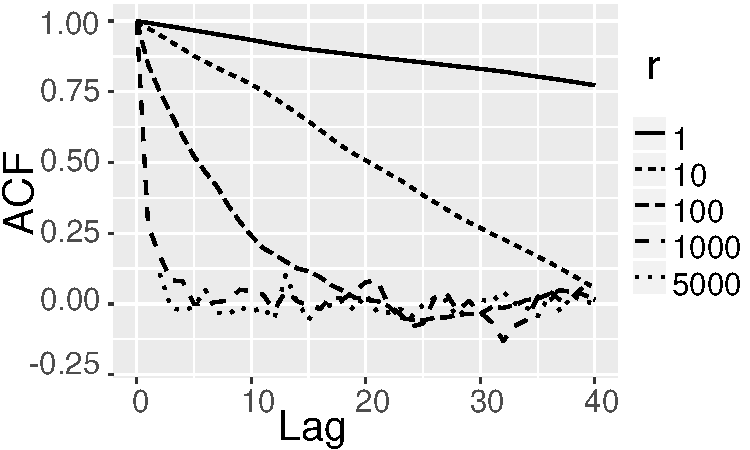
\includegraphics[width=0.3\linewidth]{probit_demo_acf_prop.pdf}}
%    \quad
    \subfigure[Posterior density estimates without MH adjustment.]{\label{probit_demo_intercept_density}
      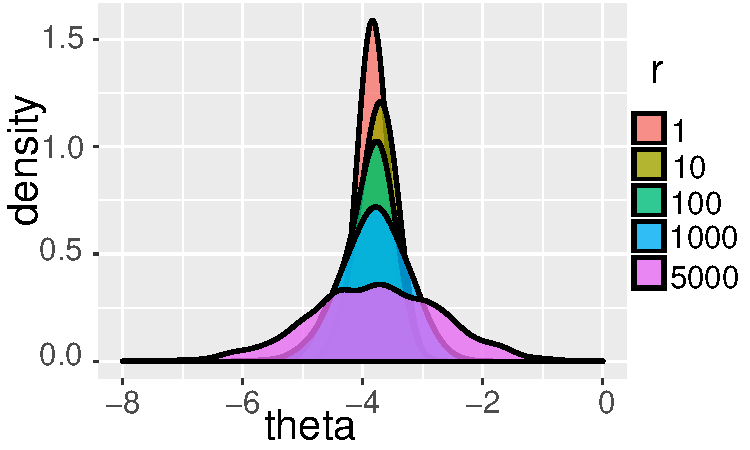
\includegraphics[width=0.3\linewidth]{density_probit.pdf}}
%    \quad
    \subfigure[ACF for CDA with MH adjustment]{
      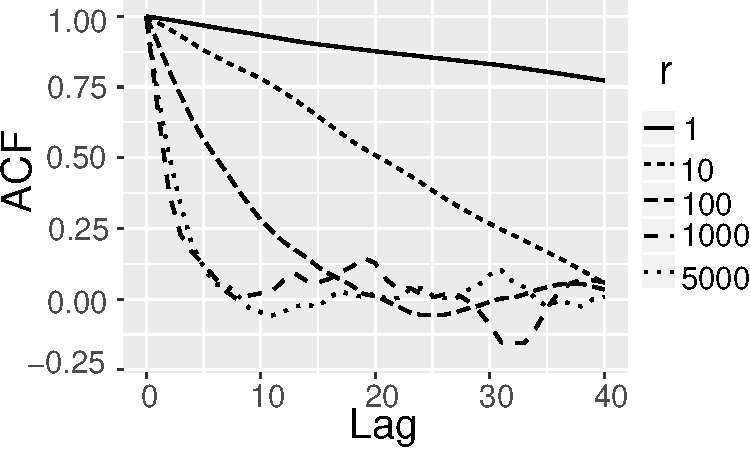
\includegraphics[width=0.3\linewidth]{probit_demo_acf.pdf}}
  }
   \label{probit_demo_intercept}
     {\caption{Autocorrelation functions (ACFs) and kernel-smoothed density estimates for different CDA samplers in intercept-only probit model.}}
\end{figure}


We also study a common hierarchical Gaussian example in appendix \ref{gaussian_example}.

\section{Specific Algorithms} \label{sec:algos}
In this section, we describe CDA algorithms for general probit and logistic regression.

\subsection{Probit Regression}
\label{probit_reg_model}
Consider the probit regression:
\be
y_i \sim \Bern(p_i), \quad p_i = \Phi(x_i \theta)  \quad i=1,\ldots,n
\ee
with improper prior $\Pi^0(\theta) \propto 1$. The data augmentation sampler \citep{tanner1987calculation, albert1993bayesian} has the update rule
\be
z_i \mid \theta, x_i, y_i &\sim \left\{ \begin{array}{cc} \No_{[0,\infty)}(x_i \theta,1) & \text{ if } y_i = 1 \\ \No_{(-\infty,0]}(x_i \theta,1) & \text{ if } y_i = 0 \end{array} \right.  \quad i=1,\ldots,n\\
\theta \mid z, x, y &\sim \No((X'X)^{-1} X'z, (X'X)^{-1}).
\ee
\cite{liu1999parameter} and \cite{meng1999seeking}, among others, previously studied this algorithm and proposed to rescale $\theta$ through parameter expansion. However, this modification does not impact the conditional variance of $\theta$ and thus does not directly increase typical step sizes.

Our approach is fundamentally different, since we directly adjust the conditional variance. Similar to the intercept only model, we modify $\mbox{var} (\theta| z)$ by changing the scale of each $z_i$. This yields the update rule
\be \label{eq:cda-probit}
z_i \mid \theta, x_i, y_i &\sim \left\{ \begin{array}{cc} \No_{[0,\infty)}(x_i \theta+b_i,r_i) & \text{ if } y_i = 1 \\ \No_{(-\infty,0]}(x_i \theta+b_i,r_i) & \text{ if } y_i = 0 \end{array} \right.  \quad i=1,\ldots,n\\
\theta \mid z, X &\sim \No((X'R^{-1}X)^{-1} X'R^{-1}(z-b), (X'R^{-1}X)^{-1}),
\ee
where $R = \diag(r_1,\ldots,r_n)$, $b = (b_1,\ldots,b_n)'$. Under the Bernoulli likelihood, we have
\be
\mbox{Pr}(y_i = 1 | \theta, x_i, r_i, b_i) & = \int_{0}^{\infty} \frac{1}{\sqrt{2 \pi r_i} } \exp\left(-\frac{(z_i-x_i\theta-b_i)^2}{2 r_i} \right) dz_i \\& = \Phi\bigg( \frac{x_i\theta+b_i}{\sqrt{r_i}}\bigg).
\label{eq:prop-marginal-probit}
\ee
For fixed $r = (r_1,\ldots,r_n)$ and $b = (b_1,\ldots,b_n)$, \eqref{eq:prop-marginal-probit} defines a proper Bernoulli likelihood for $y_i$ conditional on parameters, and therefore the transition kernel $Q_{r,b}((\theta,z);\cdot)$ defined by the Gibbs update rule in \eqref{eq:cda-probit} would have a unique invariant measure for fixed $r,b$, which we denote $\Pi_{r,b}(\theta,z \mid y)$. 
%\eqref{eq:prop-marginal-probit} suggests that another way to view CDA Gibbs is that a different link function is chosen for each observation, and the corresponding MH algorithm allows us to recover the posterior under the original link. The CDA MH algorithm in this case proposes from $Q(\theta^*;\theta) = \int f(\theta^*;z,y)  \pi(z;\theta,y) dz$, the $\theta$-marginal of the transition kernel $K_{r,b}((\theta^*,z^*);(\theta,z))$. The acceptance probability is given by \eqref{eq:MH-accrat} with $L_{r,b}(\eta_i;y_i) = \Phi\big( \frac{\eta_i+b}{\sqrt{r}}\big) ^{y_i} \Phi \big( -\frac{\eta_i+b}{\sqrt{r}}\big) ^{(1-y_i)}$; we denote $L_{1,0}$ by $L$. 

For insight into the relationship between $r$ and step size, consider the $\theta$-marginal autocovariance in a Gibbs sampler evolving according to $K_{r,b}$
\begin{equation*}
	\begin{aligned}
    &\cov_{r,b}(\theta_t \mid \theta_{t-1},X,z,y) \\
= & (X'R^{-1}X)^{-1} + (X'R^{-1}X)^{-1} X'R^{-1}\cov(z-b | R) R^{-1}X(X'R^{-1}X)^{-1} \\
\ge & (X'R^{-1}X)^{-1}. \label{eq:varlb-probit}
	\end{aligned}
\end{equation*}
In the special case where $r_i = r_0$ for all $i$, we have
\be
\cov_{r,b}(\theta_t \mid \theta_{t-1}, X,z,y) &\ge r_0 (X'X)^{-1}, 
\ee
so that all of the conditional variances are increased by at least a factor of $r_0$. This holds uniformly over the entire state space, so it follows that 
\be
\bb E_{\Pi_{r,b}}[\var(\theta_j \mid z)] \ge r_0 \bb E_{\Pi}[\var(\theta_j \mid z)]. 
\ee
The key to CDA is to choose $r,b$ to make $\bb E_{\Pi_{r,b}}[\var(\theta_j \mid z)]$ close to $\var_{\Pi_{r,b}}(\theta_j \mid z)$, while additionally maximizing the MH acceptance probability. We defer the details of tuning algorithm for $r,b$ to the next section.

For illustration, we consider a simulation study for probit regression with an intercept and two predictors $x_{i,1},x_{i,2} \sim \No(1,1)$, with $\theta=(-5,1,-1)'$, generating $\sum_i y_i\approx 20$ among $n=10,000$. The \cite{albert1993bayesian} DA algorithm mixes slowly (Figure~\ref{probit_reg_trace} and \ref{probit_reg_acf}). We also show the 
results of the parameter expansion algorithm (PX-DA) proposed by \cite{liu1999parameter}. PX-DA only mildly reduces the correlation, as it does not solve the small step size problem. After tuning, CDA reaches a satisfactory acceptance rate of $0.6$ {and leads to dramatically better mixing}. 


\begin{figure}[H]
  {%
    \subfigure[Traceplot for the original DA, parameter expanded DA and CDA algorithms.]{\label{probit_reg_trace}%
      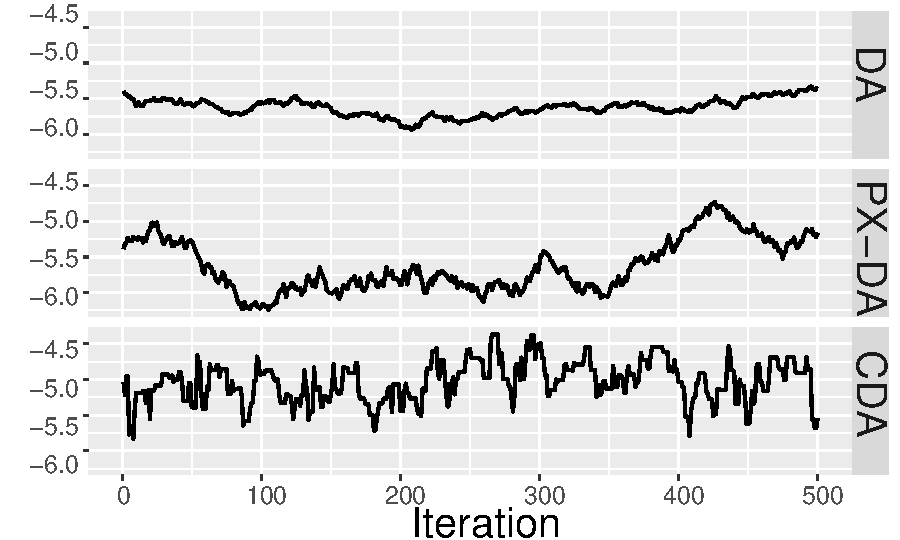
\includegraphics[width=0.45\linewidth]{probit15_trace_plot.pdf}}%
    \qquad
    \subfigure[ACF for original DA, parameter expanded DA and CDA algorithms.]{\label{probit_reg_acf}%
      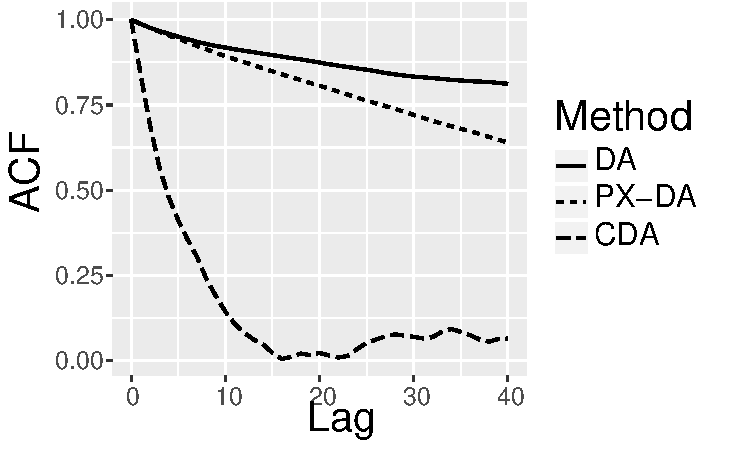
\includegraphics[width=0.45\linewidth]{probit15_acf.pdf}}
  }
 {\caption{Panel (a) demonstrates in traceplot and panel (b) in autocorrelation the substantial improvement in CDA by correcting the variance mis-match in probit regression with rare event data, compared with the original \citep{albert1993bayesian} and parameter-expanded methods \citep{liu1999parameter}.}}
\end{figure}


\subsection{Logistic Regression}
%Calibration was easy to achieve in the probit examples, because $\mbox{var}( \theta | z,y)$ does not involve the latent variable $z$.  In cases in which the latent variable impacts the variance of the conditional posterior distribution of $\theta$, we propose to stochastically increase $\mbox{var}(\theta|z,y)$ by modifying the distribution of $z$. 
In the second example, we focus on the logistic regression model with 

\begin{equation}
\label{logit_regression}
	\begin{aligned}
    y_i \sim \Bern(p_i), \quad p_i = \frac{\exp(x_i \theta)}{1+\exp(x_i \theta)} \quad i=1,\ldots,n
	\end{aligned}
\end{equation}
and improper prior $\Pi^0(\theta) \propto 1$. For this model, \cite{polson2013bayesian} proposed Polya-Gamma data augmentation:
\be
 z_i &\sim {\PG}(1, |\xtheta|) \quad i=1,\ldots,n,\\
\theta &\sim \No \left(  (X' Z X)^{-1}   X'  (y-0.5)  ,  (X' Z X)^{-1}  \right),
\ee
where $Z= \diag(z_1,\ldots,z_n)$.  This algorithm relies on expressing the logistic regression likelihood as
$$L( \xtheta; y_i )=  \int_0^\infty \exp\{ \xtheta (y_i-1/2)\} \exp\bigg\{ -\frac{z_i (\xtheta)^2}{2}\bigg\} \PG(z_i \mid 1,0) dz_i,$$
where $\mbox{PG}(a_1,a_2)$ denotes the density of the Polya-Gamma distribution with parameters $a_1,a_2$, with $\bb{E}z_i= {a_1}/{(2 a_2)}\tanh({a_2}/{2})$.

Since our goal is to increase the conditional variance $(X' Z X)^{-1}$, we can achieve this stochastically by reducing the mean $\bb{E}z_i$. 
We replace $\PG(z_i \mid 1,0)$ with $\PG(z_i \mid r_i,0)$ in the step for updating the latent data. Adding the location term $b_i$ to the linear predictor $\eta_i = x_i\theta$ leads to 
\be
L_{r,b}(\xtheta;y_i) = & \int_{0}^{\infty}  \exp\{ (\xtheta+b_i) (y_i-r_i/2)\} \exp\bigg\{ -\frac{z_i (\xtheta+b_i)^2}{2}\bigg\} \PG(z_i \mid r_i,0) dz_i \\
= &  \frac{\exp \{ (x_i \theta + b_i)y_i \}}{\{1+\exp(\xtheta +b_i)\}^{r_i}},
\label{eq:prop-marginal-logit}
\ee
and the update rule for the CDA Gibbs sampler is then 
\be
 z_i &\sim {\PG}(r_i, |\xtheta+b_i|) \quad i=1,\ldots,n,\\
\theta' &\sim \No \left(  (X' Z X)^{-1}  X'  (y -r/2- Zb) ,  (X' Z X)^{-1}  \right),
\ee
where $r = (r_1,\ldots,r_n)'$ and $b=(b_1,\ldots,b_n)'$. We again defer the tuning details for $r$ and $b$ to the next section.

For illustration, we use a two-parameter intercept-slope model with $x_{i1}\stackrel{iid}{\sim} \No(0,1)$ and $\theta=(-8,1)'$. With $n= 10^5$, we obtain rare outcome data with 
$\sum y_{i} \approx 50 $.  In CDA, after tuning, it reaches an acceptance rate of $0.8$.  Shown in Figure~\ref{logit_random_mixing}, DA mixes slowly, exhibiting strong autocorrelation even at lag $40$, while CDA has dramatically better mixing.



\begin{figure}[H]
  {%
    \subfigure[Traceplots for DA and CDA.]{%
      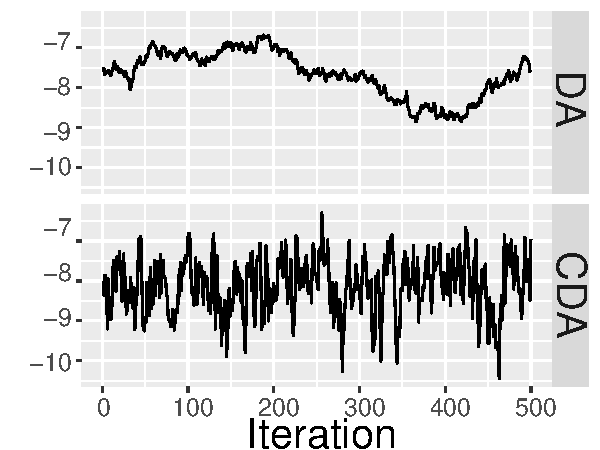
\includegraphics[width=0.45\linewidth]{traceplot_logit}}%
    \qquad
    \subfigure[ACF for DA and CDA.]{%
      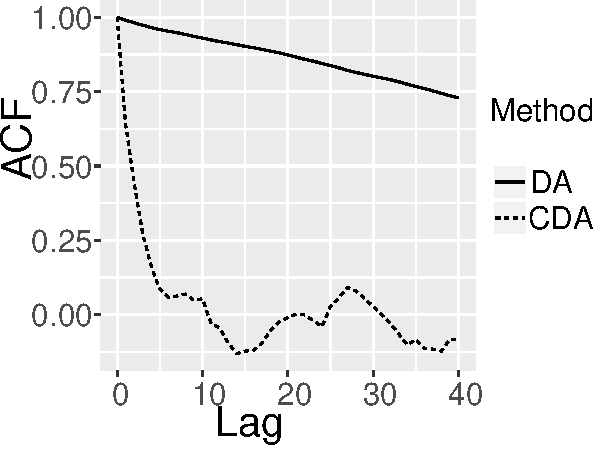
\includegraphics[width=0.45\linewidth]{acf_logit}}
  }
  {\caption{Panel (a) demonstrates in traceplot and panel (b) in autocorrelation the substantial improvement of CDA in logistic regression with rare event data, compared with the original DA \citep{polson2013bayesian}.\label{logit_random_mixing}}}
\end{figure}



\section{{Automatic Tuning of Calibration Parameters}} \label{sec:tuning}
As illustrated in the previous subsection, efficiency of CDA is dependent on good choices of the calibration parameters $r$ and $b$.  We propose a simple and efficient algorithm for calculating ``good'' values of these parameters utilizing the Fisher information and empirical MH acceptance rate.  {Although our choice of calibration parameters relies on large sample approximations, we find that this calibration approach also works well for modest sample size.}

{
Our
goal is to adjust the conditional variance under calibration of $(r,b)$ to approximately match the marginal variance under the exact target distribution, while maintaining a reasonable MH acceptance rate.

%The inverses of the following Fisher information provide  useful approximation to the two posterior covariances.

To approximate the marginal variance, we use the inverse of the observed Fisher information \citep{efron1978assessing}:
\begin{equation*}
	\begin{aligned}
		\mbox{var} (\theta \mid y) & \approx \mc I^{-1}(\hat\theta)\\
    \bigg (\mc I(\hat\theta) \bigg)_{i,j}  &  = \left( \frac{\partial}{\partial \theta_i} \log L(\theta;y) \right) \left( \frac{\partial}{\partial \theta_j} \log L(\theta;y) \right)\bigg\vert _{\theta=\hat\theta} 
	\end{aligned}
\end{equation*}
for $i=1,\ldots,p$, $j=1,\ldots,p$, where $\hat\theta$ is the Maximum a Posteriori (MAP) estimate of $\theta$.

Recall that the CDA proposal has density 
\be
q(\theta^*; \theta) = \int f_{r,b}(\theta^*;z,y)\pi_{r,b}(z; \theta,y) dz,
\ee
and the conditional variance has lower bound $\mbox{var}(\theta^*\mid \theta)\ge \mathbb{E}_{z\mid \theta} \mbox{var}(\theta^*\mid z)$. We use the inverse of the observed Fisher information to approximate $\mbox{var}(\theta^*\mid z)$ via 
\begin{equation*}
	\begin{aligned}
	 \mathbb{E}_{z\mid \theta}\mbox{var}(\theta^*\mid z) &\approx   \mathbb{E}_{z\mid \theta} \mc I^{-1}({\hat\theta};r,b,z) 
	 \approx \mc I^{-1}({\hat\theta};r,b,\tilde z(\hat\theta))	 \\
     \bigg(  \mc I({\hat\theta};r,b,z) \bigg)_{i,j}& =  \left( \frac{\partial}{\partial \theta^*_i} \log f_{r,b}(\theta^*;y,z) \right)\left( \frac{\partial}{\partial \theta^*_j} \log f_{r,b}(\theta^*;y,z) \right) \bigg\vert _{\theta^*=\hat\theta}.
	\end{aligned}
\end{equation*}
Since $\mathbb{E}_{z\mid \theta} \mathcal{I}^{-1}({\hat\theta};r,b,z)$ is often intractable or cumbersome to compute, we instead use the second approximation, the Fisher information evaluated at $\tilde z(\hat\theta)$, the conditional mean or mode of $\pi_{r,b}(z;\hat\theta,y)$. The choice between mean and mode depends on which has a closed-form expression.

One can now adjust $r,b$ to reduce the distance
\begin{equation}
\label{variance_dist}
	\begin{aligned}
    d_1(r,b)= \Dist \bigg[\mc I^{-1}(\hat \theta), \mc I^{-1}({\hat\theta};r,b,\tilde z(\hat\theta)) \bigg],
	\end{aligned}
\end{equation}
where $\Dist(M_1,M_2)$ is a distance between two matrices, such as $\|M_1-M_2\|_F$ or $\|M_1^{-1}-M_2^{-1}\|_F$, the Frobenius norm of the difference.

However, the increase in proposal variance only results in an increase in the variance of the Metropolis-Hastings transition density so long as the acceptance probability is not substantially depressed (relative to the DA Gibbs sampler, which has acceptance probability one). Therefore, one also needs to adjust $(r,b)$ both to optimize the acceptance rate $\alpha(\theta,\theta^*)$ and the proposal variance. Considering the average acceptance rate (on the negative-log scale), with expectation over proposal density $q(\theta^* ; \theta)$ and posterior  $\pi(\theta\mid y)$
\begin{equation*}
	\begin{aligned}
  & \mathbb{E}_{\theta\mid y}\mathbb{E}_{\theta^*\mid\theta} \big[-\log\alpha(\theta,\theta^*) \big]    \\=&
   \mathbb{E}_{\theta\mid y}\mathbb{E}_{\theta^*\mid z} \mathbb{E}_{z\mid \theta}    \max \bigg[ -\log\frac{L(\theta^*;y)}{L_{r,b}(\theta^*;y)} +
  \log\frac{L(\theta;y)}{L_{r,b}(\theta;y)},0\bigg].
  \end{aligned}
\end{equation*}
To provide tractable computation, we again use the functions evaluated at the conditional mean or mode to approximate the three expectations. This yields
\begin{equation}
\label{acceptance_dist}
	\begin{aligned}
d_2(r,b)  =&  \max \bigg[ -\log\frac{L(\tilde \theta^*(\tilde z(\hat\theta));y)}{L_{r,b}(\tilde \theta^*(\tilde z(\hat\theta));y)} +
  \log\frac{L(\hat\theta;y)}{L_{r,b}(\hat\theta;y)},0\bigg],\\
	\end{aligned}
\end{equation}
with $\hat\theta$ the MAP of $\theta$,  $\tilde z(\theta)$ the mean or mode of $\pi_{r,b}(z;\theta,y)$,  $\tilde \theta^*$ the mean or mode of $f_{r,b}(\theta^*;z,y)$.

Combining  \eqref{variance_dist} and \eqref{acceptance_dist}, this yields the optimal tuning parameters under those two criteria:
\begin{equation}
\label{tuning_objective_function}
	\begin{aligned}
(\hat r,\hat b) =  \min_{r,b}  \big[d_1(r,b) + \lambda d_2(r,b)\big].
	\end{aligned}
\end{equation}
The optional parameter $\lambda>0$ allows for differential weighting of the acceptance rate and variance, although the default $\lambda=1$ works well for all of our applications.

To facilitate automatic tuning in generic cases, we exploit the automatic differentiation and  optimization software, TensorFlow, to compute the Fisher information and optimize for $(\hat r, \hat b)$. One only needs to provide the densities $L_{r,b}(\theta;y)$, $f_{r,b}(\theta^*;z,y)$, $\pi_{r,b}(z;\theta,y)$ and two conditional estimators $\tilde z(\theta)$ and $\tilde \theta^*(z)$.

We now provide the tuning details for probit and logistic regression. The likelihood and update densities $L_{r,b}(\theta;y)$, $f_{r,b}(\theta^*;z,y)$, $\pi_{r,b}(z;\theta,y)$ are already given, we present the conditional estimators. For probit regression, the two conditional modes for $\pi_{r,b}(z;\theta,y)$,  $\tilde \theta^*$ and $f_{r,b}(\theta^*;z,y)$  are available in closed form, viz
\begin{equation*}
	\begin{aligned}
    \tilde z_i(\theta) = & \left\{ 
    \begin{array}{lll}
         & x_i\theta +b_i &\text{if } (y_i-0.5)  (x_i\theta +b_i)>0\\
         & 0 &\text{otherwise}
    \end{array} \right. \text{ for } i=1,\ldots,n, \\
    \tilde \theta^*(z) = & (X'R^{-1}X)^{-1} X'R^{-1}(z-b).
	\end{aligned}
\end{equation*}

For logistic regression, the conditional means for $\pi_{r,b}(z;\theta,y)$,  $\tilde \theta^*$ and $f_{r,b}(\theta^*;z,y)$ all have closed-form expressions given by
\begin{equation*}
	\begin{aligned}
    \tilde z_i(\theta) = &  \frac{r_i}{2|x_i\theta_i+b_i|} \tanh(\frac{|x_i\theta_i+b_i|}{2}) \quad i=1,\ldots,n, \\
    \tilde \theta^*(z) = & (X' Z X)^{-1}  X'  (y -r/2- Zb).
	\end{aligned}
\end{equation*}



{
\section{Geometric convergence rates for CDA-MH and CDA-Gibbs}
}
Although Remark \ref{rem:ergodic} gives a basic guarantee of convergence of the usual time-averaging estimators commonly used in MCMC, the goal of CDA-MH is to improve upon the convergence rate of the usual DA Gibbs. Motivation for CDA is provided by the results of \cite{johndrow2016inefficiency}, which studied the special case of intercept-only logistic and probit regression when $y=1$ and $n \to \infty$ so that the data grow increasingly imbalanced as the sample size increases. \citet{johndrow2016inefficiency} showed that in this setting, the spectral gap of DA converges to zero at least as fast as $n^{-1/2} (\log n)^k$ for $k \le 5.5$, while random-walk Metropolis has spectral gap order $(\log n)^3$ or larger. This suggests the superiority of Metropolis algorithms in the large sample imbalanced data setting. However, to implement Metropolis effectively with moderate to large numbers of covariates, one needs an efficient way to construct proposals, which is the goal of CDA.

We now give a result on the convergence rates of CDA and CDA-MH for imbalanced intercept-only logistic regression. The result shows that the spectral gap is larger than that for DA (as a function of $n$), and comparable to MH with optimally tuned proposals when $y$ grows no faster than $\log n$. While this is a special case, we note that the result in \cite{johndrow2016inefficiency} is given only for fixed $y=1$, and thus our result is more general. The difficulty of obtaining quantitative estimates of the rate at which the spectral gap converges to zero as $n$ grows is underscored by the length and complexity of the arguments in \citet{johndrow2016inefficiency}. 

%We now provide some theory regarding the geometric convergence of CDA-MH algorithm. Assuming the original DA-Gibbs algorithm is uniformly ergodic, its Markov transition density $q(\theta,\theta')$ has a minorization condition:
%
%\begin{equation*}
%	\begin{aligned}
%    & q(\theta,\theta') \ge \kappa p(\theta') \quad \forall (\theta,\theta')\in \Theta\times \Theta
%	\end{aligned}
%\end{equation*}
%where $p(\theta')$ is a probability density and a constant $\kappa>0$, commonly known as the spectral gap.
%
%Letting $\Pi(.)$ be the invariant measure and ${Q}^t(.;\theta_0)$ be the $\theta$-marginal measure after transitioning via $q(\theta';\theta)$ for $t$ iterations from an initial state $\theta_0$. The convergence rate can be expressed in the form of a geometric upper bound
%
%\begin{equation*}
%	\begin{aligned}
%    \|\Pi(.),{Q}^t(.;\theta_0)\|_{TV} \le (1-\kappa)^t,
%	\end{aligned}
%\end{equation*}
%where $\|.\|_{TV}$ is the total variation distance.
%
%However, for the considered DA-Gibbs algorithms, the spectral gap $\kappa$ decreases rapidly to $0$ as $n$ increases. For example, in logistic regression, the spectral gap approaches $0$ in $\kappa=\mc O(n^{-1/2})$ when $\sum_i y_i\ll n$\citep{johndrow2016inefficiency}. This bound would not provide any meaningful convergence guarantee under large $n$. 
%
%The advantage of the CDA-MH is that $\kappa$ becomes tunable as a function of $r,b$. One could adjust them to reduce the effect of $n$, leading to more effective convergence bound. 
%
%To theoretically quantify the improvement, we study the logistic regression with intercept case.
Consider intercept-only logistic regression
from \eqref{logit_regression} with $x_i =1$ for $i=1,\ldots,n$ and prior $\theta\sim \No(0, \sigma^2)$.
%\begin{equation*}
%	\begin{aligned}
%    y_i \sim \Bern(p_i), \quad p_i = \frac{\exp(\theta)}{1+\exp(\theta)} \quad i=1,\ldots,n, \quad \theta\sim \No(0, \sigma^2)
%	\end{aligned}
%\end{equation*}
As all $p_i$'s are the same, we use a single scalar $r_i=r$  and $b_i=b$ for all $i$. With $r,b$ fixed, the update rule for CDA-Gibbs is
    \be
    \pi_{r,b}(z \mid \theta) &= {\PG}(nr, |\theta+b|) \\
    f_{r,b}(\theta'\mid z) &= \No(  m, \Lambda  )
    \ee
where $ \Lambda= { ( z + 1/\sigma^2)}^{-1} $, $m = \Lambda a -b$ and $a= \sum_i y_i - nr/2 +b/\sigma^2$.

\begin{theorem}
Consider intercept-only logistic regression with $n$ observations. Then
\begin{enumerate}
\item CDA-Gibbs is uniformly ergodic
\item CDA-MH is uniformly ergodic
\item If $\sum_i y_i = o(\log n)$, there exist choices for $r,b$ such that CDA-MH has spectral gap
\be
\kappa = \bigO(n^{-\frac{2.5+2 \log 2}{\sigma^2}}).
\ee
\end{enumerate}
\end{theorem}
Thus, for $\sigma^2> 5+4 \log 2 \approx 7.77$, the spectral gap of CDA-MH goes to zero more slowly with increasing $n$ than DA-Gibbs. Moreover, if we choose the prior $\sigma^2 = \log n$, the spectral gap of CDA-MH is independent of $n$. It follows that CDA-MH mixes rapidly as $n \to \infty$ in the large-sample imbalanced setting, unlike DA-Gibbs, which has spectral gap converging to zero at rate $n^{-1/2}$ or faster (ignoring logarithmic factors).

To show that the result is borne out empirically, we conduct simulations as in \cite{johndrow2016inefficiency}, 
with fixed $\sum_i y_i=1$ and increasing $n$ from $10^1$ to a massive $10^{14}$.  
Figure~\ref{massive_n_sims} compares the effective sample size per $1,000$ steps using DA and CDA. The deterioration of DA shows up as early
as $n=10^2$; its slow-down becomes critical at $n=10^4$ with effective sample size close to $0$. CDA performs exceptionally well, even at $n=10^{14}$ (we stop at $10^{14}$ as $1/n$ reaches the limit of floating point accuracy).\begin{figure}[H]
  \centering
       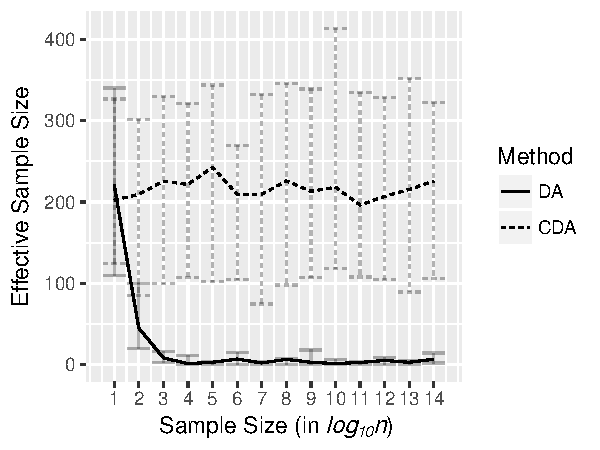
\includegraphics[width=0.6\linewidth]{simMassiveN}
         {\caption{Effective sample size (with 95\% pointwise confidence interval) per $1,000$  steps  with different sample  size $n$ from $10$ to $10^{14}$, using logistic regression model with intercept.   \label{massive_n_sims}}}
\end{figure}


\section{Simulation Study}


In this section, we compare the performance of CDA against popular alternative algorithms.

\subsection{Comparison with Downsampling Algorithm}
\label{sec:down_sampling}
As motivated in the introduction,  two factors are necessary for MCMC to be practically useful: a low computing cost  in each iteration and a high effective sample size within a small number of iterations. 

One potential issue for data augmentation in general is the large number of latent variables to sample in each iteration.  A common strategy is to {avoid sampling latent variables for
every observation by approximating the Markov transition kernel using subsamples} 
\citep{korattikara2014austerity,quiroz2016exact, bardenet2017markov}.  {Unlike other
alternative algorithms we consider here, this changes the invariant measure. Finding
a suitable sub-sample size while controlling the approximation
error is challenging and usually problem-specific \citep{johndrow2015approximations, rudolf2018perturbation}, and we do not consider it here. Instead, our goal is to show sub-sampling alone does not address the low ESS of DA; whereas }{one can trivially combine our proposed CDA
strategy with subsampling to scale DA-MCMC up to enormous data sample sizes.  We illustrate this strategy here.}

We consider the same two-parameter intercept-slope model in logistic regression
as described above, except we now vary data sample size from  $n=10^5$ to $10^8$. We simulate Bernoulli outcomes $y_i\sim \Bern\big(({1+\exp(-x_i\theta)})^{-1}\big)$ with $x_i=(1,w_i)$ for $w_i \stackrel{iid}{\sim} \No(0,1)$ and $\theta=(-\theta_0,1)'$. We vary $\theta_0$ to obtain $\sum{y_i} \approx
10$ for each $n$. We utilize the minibatch Polya-Gamma algorithm described by \cite{johndrow2015approximations},
and apply CDA to calibrate the variance discrepancy. Since $y$ is highly imbalanced, we apply biased sampling by including all data
with $y_i=1$, while sub-sampling $1\%$ of data with $y_i=0$. %{Existing work on applying biased subsampling in logistic regression mainly aims to obtain point estimates \citep{king2001logistic,wang2017optimal},
%in this article we present a simple solution for Bayesian inference.}

Denoting the set of all data with $y_i=1$ as $V_1$ and a random subset  with $y_i=0$ as $V_0$, we adjust the likelihood contribution from $y_i=0$ via a power of $({n-|V_1|})/{|V_0|}$ to compensate for the downsampling, leading to an approximate likelihood
$$L(\theta;y) = \prod_{i\in V_1}\frac{\exp(x_i\theta)}{ 1+\exp(x_i\theta)} \left (\prod_{i\in V_0}\frac{1}{ 1+\exp(x_i\theta)}
\right)^{\frac{n-|V_1|}{|V_0|}}.$$
The number of latent variables is reduced to $n_0 \equiv |V_0|+|V_1|$; since
$n_0$ is still large, slow mixing remains a problem and calibration is needed. The algorithmic details are presented in the appendix.


Figure~\ref{simMassiveNSubsampling} compares the performance of the two approximating
algorithms, one  combining CDA and sub-sampling, and one  using sub-sampling alone. Clearly, sub-sampling alone still results in very small
effective sample size, while using CDA and sub-sampling together can produce excellent computational performance.
\begin{figure}[H]
\centering
  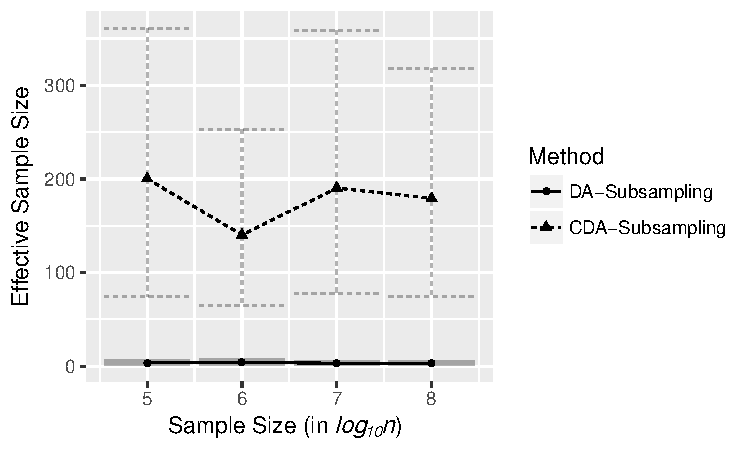
\includegraphics[width=0.55\linewidth]{simMassiveNSubsampling}
    {\caption{Comparing the performance of CDA and DA, coupled with sub-sampling
 approximation to reduce the number of sampled latent variables. \label{simMassiveNSubsampling}}} %Only accelerating computing time in each iteration (DA-Subsampling) does not solve the scalability issue.      
\end{figure}

\subsection{Comparison with Independence Metropolis-Hastings}
In the CDA-MH algorithm, we utilize the marginal quantities $\hat \theta$ and $\mc I(\hat\theta)$ to tune the $(r,b)$ parameters. We compare the performance of the CDA proposal against alternative MH proposal with access to the same information. Specifically, we analyze MH using independent multivariate $t$ proposals with mean $\hat \theta$ and variance $\mc I^{-1}(\hat\theta)$. We show that this algorithm has very low acceptance rate relative to CDA-MH.

The general form of the MH acceptance rate is given by
\begin{equation*}
	\begin{aligned}
    \alpha(\theta,\theta^*) = \min\bigg\{ 1, \frac{L(\theta^*;y)q(\theta;\theta^*)}{q(\theta^*;\theta)L(\theta;y)} \frac{\Pi^0(\theta^*)}{\Pi^0(\theta)}\bigg\}.
	\end{aligned}
\end{equation*}
Assuming the prior $\Pi^0(\theta)$  has negligible impact when $n$ is large, the key to a high acceptance rate is to have $L(\theta;y)/q(\theta;\theta^*)$ close to a constant in the high posterior density region of the parameter space. However, for computational convenience, one often has to use a proposal that is easy to sample. The density mis-match between $L(\theta;y)$ and $q(\theta;\theta^*)$  can cause the ratio to decrease rapidly moving away from the posterior mode of $\theta$,  resulting in a high rejection rate.

To illustrate, we consider the independent multivariate $t$-distribution proposal for logistic regression:
\begin{equation*}
	\begin{aligned}
    q(\theta^*,\theta)=q(\theta) = t_{\nu} \left\{ \theta ; \hat\theta, (\nu-2){\nu}^{-1} \mathcal{I}^{-1}(\hat\theta) \right\},
	\end{aligned}
\end{equation*}
where $\nu>2$ and $\mathcal{I}(\hat\theta)= X^{T} \diag[ \exp(x_i\hat\theta) \{ 1+\exp(x_i\hat\theta) \}^{-2} ] X$. The second parameter is set to have $\mbox{var}(\theta)=\mathcal{I}^{-1}(\hat\theta)$ exactly. We choose $\nu=3$ to induce a tail heavier than the target likelihood, which is a necessary condition for geometric ergodicity of MH with independent proposals \citep{mengersen1996rates}.

The density ratio is
\begin{equation}
\label{eq:density_ratio_indep_proposal}
	\begin{aligned}
&    \frac{L(\theta;y)}{q(\theta)} =  c_1\left \{ \prod_i \frac{ \exp(y_i x_i\theta )}{1+\exp( x_i\theta)} \right \}\left \{ 1+\frac{1}{\nu-2} (\theta-\hat\theta )^{\rm T}{\mathcal{I}(\hat\theta)} (\theta-\hat\theta ) \right\}^{(\nu+p)/2} \\
   &  \quad =  c_1  \frac{  \exp(\sum_i y_i x_i\theta )}{  \prod_i \{ 1+\exp( x_i\theta)\}}   \left [ 1+ \sum_i \frac{1}{\nu-2} (x_i \theta-x_i \hat\theta  )^2  \exp(x_i\hat\theta) \{ 1+\exp(x_i\hat\theta) \}^{-2} \right ]^{(\nu+p)/2},
	\end{aligned}
\end{equation}
where  $c_1$ denotes the constant part. We give an approximation of the acceptance ratio.

We focus on the case $\sum y_i \ll n$, where  the mixing is slow for DA-Gibbs.  This results in $\exp(x_i\hat\theta)\approx 0$ for most $i$.  Assuming the high posterior density region is a neighborhood $\{ \theta:|x_i \theta-x_i \hat\theta  |< \eta \;\text{ for all } i \}$, where $\eta$ is a bounded constant, the second term in \eqref{eq:density_ratio_indep_proposal} is close to a constant, while the first term is approximately equal to its numerator. The acceptance ratio is thus approximately
\begin{equation*}
	\begin{aligned}
	\frac{L(\theta^*;y)q(\theta)}{q(\theta^*)L(\theta;y)}
	  \approx  \exp \left \{   \sum_i y_i x_i (\theta^* - \theta ) \right\},
    \end{aligned}
\end{equation*}
 which decreases exponentially away from the current state. 
 
% \jjtodo{I'm still confused about what we're saying here. If we move toward the mode, then the acceptance ratio is 1, since the proposal is symmetric. Isn't it? }
%\ldtodo{\@James, the acceptance ratio  isn't $1$ at the mode. Because the proposal is not centered at the current value, therefore is asymmetric $q(\theta\mid \hat\theta, \mc{I}^{-1}) \neq q(\theta'\mid \hat\theta, \mc{I}^{-1})$}
%\jjtodo{It seems what is really going on with CDA vs MH is that (1) if we use a t proposal constructed with the fisher info, it typically won't be a good approximation to the target and (2) if we use gaussian random walk metropolis, it will perform badly as dimension increases. Seems we could argue for this without necessarily making sketchy looking approximations to the acceptance ratio, while backing up our arguments with empirical analysis.}

In contrast, since the CDA proposal density is similar to the target, with calibration the density ratio can be made close to a constant in the neighborhood of the mode. Consider the density ratio in the logistic CDA proposal:
\begin{equation*}
	\begin{aligned}
    \frac{L(\theta;y)}{L_{r,b}(\theta;y)} =
    c_2 \prod_i \frac{ \{ 1+\exp( x_i\theta+b_i)\}^{r_i}}{1+\exp( x_i\theta)},
    \end{aligned}
\end{equation*}
where $c_2$ is a constant.  Minimizing the Fisher information distance gives approximately $r_i\approx\exp(x_i\hat\theta)$ and $b_i \approx -x_i\hat\theta$, so the density ratio is approximately $c_2$. Thus the acceptance ratio
\begin{equation*}
	\begin{aligned}
	\frac{L(\theta^*;y)L_{r,b}(\theta;y)}{L_{r,b}(\theta^*;y)L(\theta;y)}
	  \approx  1.
    \end{aligned}
\end{equation*}


{ We compare the performance of MH algorithms with $t_3$ and CDA proposals, using the two-parameter intercept-slope example  described in Section \ref{sec:down_sampling}. Figure~\ref{acceptance_rate_tail} shows the acceptance ratio at different intercept values $\theta_0$, which is approximately the average of $x_i\theta$. The acceptance rate drops rapidly to $0$ for the $t_3$ proposal, and is close to one for the CDA proposal.}
 \begin{figure}[H]
 \begin{center}
     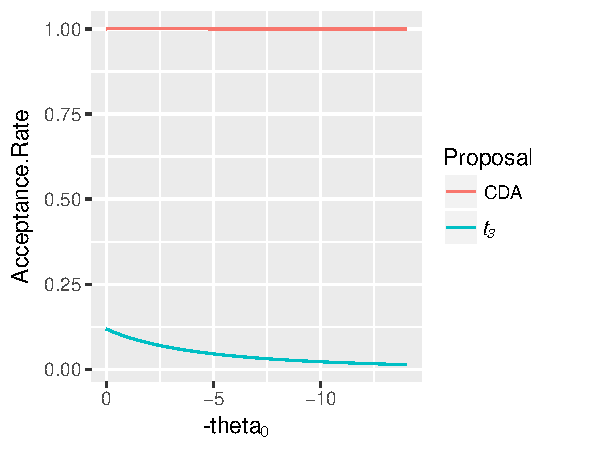
\includegraphics[width=0.6\linewidth]{acceptance_rate_mhs2}
 \end{center}
    {\caption{Comparing the acceptance ratios using the multivariate $t$-distribution and CDA proposals in logistic regression, with variance fixed at the inverse Fisher information. CDA has a much higher acceptance ratio than the multivariate $t$ proposal.\label{acceptance_rate_tail}}}
\end{figure}





 \section{Data Applications}


\subsection{{Bernoulli Latent Factor Model with Group Intercepts for Network Modeling}}

We now apply CDA to accelerate estimation of group intercepts in a latent factor model. The dataset is  a large sparse network from the Human Connectome Project \citep{marcus2011informatics}. The network data under consideration is an adjacency matrix representing the connectivity among $V=1015$ macroscopic regions of one human brain. The matrix $\{A_{ij}\}_{(i,j) \in\{1\ldots V\}^2}$ is binary and symmetric. For $i\neq j$, $A_{ij}=1$ if regions $i$ and $j$ are connected, $A_{ij}=0$ otherwise; $A_{ii}$ are missing as self-connections are ignored. Therefore, there are effectively $n= V(V-1)/2=514,605$ observed binary outcomes.

There are $507$ regions located in the left ($\mathcal{L}$) and $508$ in the right hemisphere ($\mathcal{R}$). There are many more connections within each hemisphere ($ \sum A_{i\in \mathcal{L}, j \in \mathcal{L}, i>j} = 2,280$, $\sum A_{i\in \mathcal{R}, j \in \mathcal{R}, i>j}$ $=2,443$), than across hemispheres ($\sum A_{i\in \mathcal{L}, j \in \mathcal{R}} = 23$). To quantify this phenomenon, we use two intercepts $\beta_0$ and $\beta_1$ to represent the within- and across-hemisphere fixed effects within the following Bernoulli probit latent factor model
\begin{equation*}
	\begin{aligned}
    & A_{ij} \sim   \Bern(p_{ij}), \qquad p_{ij}=\Phi(\psi_{ij}), \\
    & \psi_{ij} =\sum_{r=1}^d u_{ir} v_r u_{jr} + \beta_{0} w_{ij} + \beta_{1} (1-w_{ij})  \quad \text{ for } i=2\ldots V, j < i,\\
%    & \Psi = UVU^T + \beta_0 W + \beta_1 (J-W) ,\\
    & \pi(U)\propto 1, \qquad U^{\rm T}U =I_d,\\
    & v_r\sim \No_{(0,\infty)}(0, \sigma^2) \qquad \text{ for } r=1,\ldots,d,\\
    & \beta_0\sim \No(0,100), \quad \beta_1\sim \No(0,100),\quad \sigma^2\sim \IG(2,1),\\
	\end{aligned}
\end{equation*}
where $w_{ij}=0$ if $i\in \mathcal{L}$ and $j\in \mathcal{R}$, otherwise $w_{ij}=1$; $U=\{u_{ir}\}$ is a $V$-by-$d$ matrix of latent factors. Following \cite{hoff2009simulation}, we assign $U$ a uniform prior on Stiefel manifold $\bb{S}^{V\times d}=\{U:U^{\rm T}U=I_d\}$, and set the latent dimension at $d=10$. The latent variable updates in the probit data augmentation algorithm are given by
\begin{equation*}
	\begin{aligned}
  &   z_{ij}\sim \left\{
    \begin{array}{lcc}
         \No_{(0,\infty)}(\psi_{ij},1) & \text{ if } A_{ij}=1 \\
         \No_{(-\infty,0)}(\psi_{ij},1)& \text{ if } A_{ij}=0 \\
    \end{array}\right. \quad \text{ for } i=2\ldots V, j<i,\\
  &  z_{ji}=z_{ij}.\\
%& z_{ii}   \sim \No(\psi_{ii},2).
	\end{aligned}
\end{equation*}

Because the connection data are highly imbalanced -- fewer than 5,000 connections out of a possible 514,605 -- the intercepts $\beta_0$ and $\beta_1$ mix slowly in an ordinary DA Gibbs algorithm (Figure~\ref{fig:network_model}(a)).   Without using DA, efficient MH proposals are difficult to develop due to the restriction that $U\in\bb{S}^{V\times d}$. The DA-Gibbs relies on the full conditional distribution
\begin{equation*}
	\begin{aligned}
    U\mid \beta_0,\beta_1,Z \sim \text{Bingham}( \{z_{ij}- \beta_0w_{ij}-\beta_1(1-w_{ij}) \}, \diag\{v_r/2\}).
	\end{aligned}
\end{equation*}


\begin{figure}[H]
  {
    \subfigure[ACFs of the parameters  $\beta_0$ and $\beta_1$ using DA.]{
      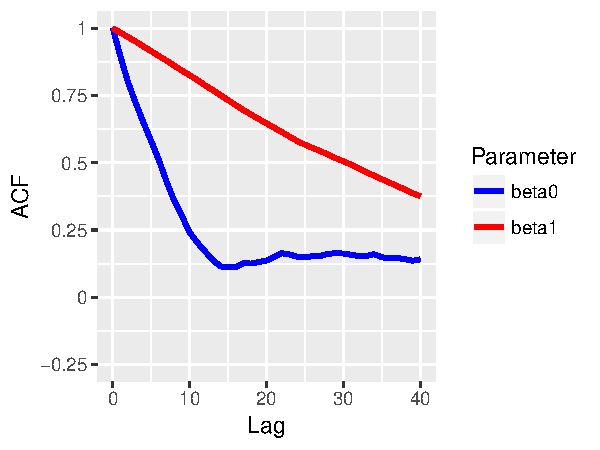
\includegraphics[width=0.45\linewidth]{acf_network_da}}
    \qquad
    \subfigure[ACFs of the parameters  $\beta_0$ and $\beta_1$ using CDA.]{
      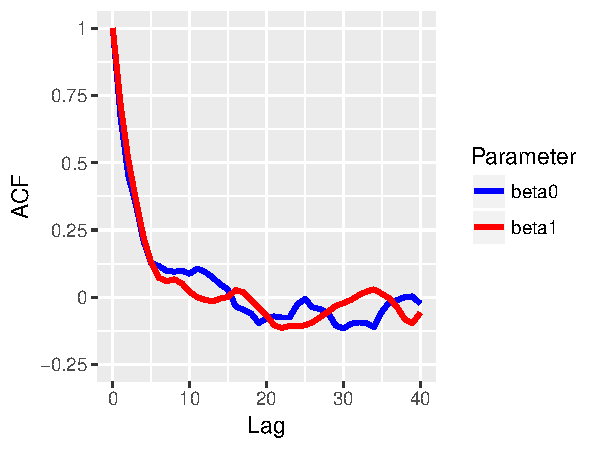
\includegraphics[width=0.45\linewidth]{acf_network_cda}}
  }
    {\caption{ACFs show the mixing performance of $\beta_0$ and $\beta_1$ in modeling average sparsity in network connectivity of a brain. \label{fig:network_model}}}
\end{figure}
We use CDA to calibrate the updates of $\beta_0$ and $\beta_1$, while keeping the other Gibbs sampling steps unchanged, i.e.
\begin{equation*}
	\begin{aligned}
     z^*_{ij} & \sim \left\{
    \begin{array}{lcc}
         \No_{(0,\infty)}(\psi_{ij}+b_{ij},r_{ij}) & \text{ if } A_{ij}=1 \\
         \No_{(-\infty,0)}(\psi_{ij}+b_{ij},r_{ij})& \text{ if } A_{ij}=0 \\
    \end{array}\right. \quad \text{ for } i=2\ldots V, j<i,\\
        \beta^*_0 & \sim \No \bigg(  [\sum_{j<i}\frac{w_{ij}}{r_{ij}}]^{-1}\sum_{j<i}\big[\frac{w_{ij}}{r_{ij}}(z^*_{ij}-b_{ij}-\sum_{r=1}^d u_{ir} v_r u_{jr})\big], [\sum_{j<i}\frac{w_{ij}}{r_{ij}}]^{-1} \bigg), \\
    \beta^*_1 & \sim \No \bigg(  [\sum_{j<i}\frac{1-w_{ij}}{r_{ij}}]^{-1}\sum_{j<i}\big[\frac{1-w_{ij}}{r_{ij}}(z^*_{ij}-b_{ij}-\sum_{r=1}^d u_{ir} v_r u_{jr})\big], [\sum_{j<i}\frac{1-w_{ij}}{r_{ij}}]^{-1} \bigg).
	\end{aligned}
\end{equation*}
Then $\beta^*_0$ and $\beta^*_1$ are accepted via MH step with calibrated conditional density 
\begin{equation*}
	\begin{aligned}
    &L_{r,b}(\beta_0,\beta_1 \mid U,V,A) = \prod_{j<i}\Phi(\psi_{ij})^{A_{ij}} [1-\Phi(\psi_{ij})]^{(1-A_{ij})}\\
    & \psi_{ij} =r_{ij}^{-1} [ \sum_{r=1}^d u_{ir} v_r u_{jr} + \beta_{0} w_{ij} + \beta_{1} (1-w_{ij}) + b_{ij}]
	\end{aligned}
\end{equation*}
The tuning parameters are optimized using the approach described in Section~\ref{sec:tuning}, except with $x_i\theta$ replaced by $\sum_{r=1}^d u_{ir} v_r u_{jr} + \beta_{0} w_{ij} + \beta_{1} (1-w_{ij})$.
%To be clear, the augmented $z^*_{ij}$ under calibration is only used for updating $\beta_0$ and $\beta_1$. Although this involves generating extra random variables in addition to $z_{ij}$, such cost is negligible in computing time per iteration (Row 4 in Table~\ref{table:network}).

\begin{table}[H]
\small
\centering
\begin{tabular}{|l |r |r| r| } 
 \hline
                          & DA & CDA \\
 [0.5ex]
$ \beta_0$         &  -2.09 (-2.10, -2.08) &  -2.09 (-2.10, -2.08)   \\
$ \beta_1$         &  -3.68 (-3.72, -3.64)&  -3.75 (-3.86, -3.66)   \\
Fitted AUC              & 90.5\% & 92.1\%\\
$T_{eff} / T$ & 0.008  & 0.142 \\
Avg Computing Time /  $T$  & 2.0 sec       & 2.0 sec       \\
Avg Computing Time /  $T_{eff}$  & 251 sec       & 14.1 sec        \\
 \hline
\end{tabular}
\caption{Parameter estimates and computing speed of DA and CDA in Bernoulli latent factor modeling of a brain network.}
\label{table:network}
\end{table}

We run DA for $30,000$ steps and CDA for $2,000$ steps, so that they have approximately the same effective sample size (calculated with the \texttt{CODA} package in \texttt{R}). Both algorithms are initialized at the MAP estimates. CDA leads to significant reduction in autocorrelation (Figure~\ref{fig:network_model}(b)) and about $18$ times lower computing time per effective sample size. We also compare the {in-sample} fitted AUCs, computed based on $A_{ij}$ and the posterior mean of $p_{ij}$. The CDA estimates clearly have a better fit to the data.

%\subsection{Hierarchical Binomial Model for Co-Browsing Rates}
%
%We initially focus on one client website and analyze co-browsing rates with the high-traffic sites. With the total visit count $N_i$ available for the $i$th high-traffic site, the count of co-browsing $y_i$ can be considered as the result of a binomial trial. With $y_i$ extremely small relative to $N_i$ (ratio  $0.00011 \pm  0.00093$), the maximum likelihood estimate $y_i/N_i$ can have poor performance. For example, when $y_i=0$, estimating the rate as exactly $0$ is not ideal. Therefore, it is useful to consider a hierarchical model to allow borrowing of information across high-traffic sites:
%\be
%y_i \sim \Binom\left(N_i, \frac{\exp(\theta_i)}{1+\exp(\theta_i)}\right), \quad \theta_i\stackrel{iid}{\sim} \No(\theta_0, \sigma^2_0), \quad i=1\ldots n\\
%(\theta_0,\sigma^2_0) \sim  \pi(\theta_0,\sigma^2_0) 
%\ee
%{We choose  weakly informative priors}. Based on expert opinion in quantitative advertising, we use a prior $\theta_0\sim \No(-12,49)$ and uniform prior on $\sigma^2_0$. Similar to the logistic regression, we calibrate the binomial Polya-Gamma augmentation, leading to the proposal likelihood:
%\be
%L_{r,b}(\theta_i;y_i,N_i, r_i, b_i) = \frac{\exp(\theta_i+b_i)^y_i}{\{ 1+\exp(\theta_i+b_i)\}^{N_ir_i}}
%\ee
%
%Conditioned on the latent Polya-Gamma latent variable $z_i$, each proposal $\theta^*_i$ can be sampled from:
%\be
%z_i &\sim \PG\left( (N_ir_i),\theta_i+b_i \right),\\
%\theta_i^* &\sim \No \left( \frac{ y_i - r_i N_i/2 -z_i b_i + \theta_0/\sigma^2_0}{z_i+ 1/\sigma^2_0}, \frac{1}{z_i+ 1/\sigma^2_0}\right),
%\ee
%and accepted or rejected using an MH step. We further require $r_i \ge (y_i-1)/N_i + \epsilon$ to have a proper $L_{r,b}(\theta_i;y_i, N_i)$ with $\epsilon$ a small constant. Similar to logistic regression, the auxiliary parameters are chosen as 
%\be
%r_i & =\frac{\exp(\theta_i)}{ \{1+\exp(\theta_i)\} ^2} / \left (   \frac{1}{2 |\theta_i+b_i|} \tanh\frac{|\theta_i+b_i|}{2} \right) \vee \big ( (y_i-1)/N_i + \epsilon \big),\\
%b_i &=\log[  \{1+\exp(\theta_i)\}^{1/r_i} -1] - \theta_i\ee
%during adaptation. Since $\theta_i$'s are conditionally independent, the calibrated proposal can be individually accepted with high probability for each $i$. This leads to a high average acceptance of $0.9$, despite the high dimensionality of $59,792$ $\theta_i$'s.
%After $\theta_i$'s are updated, other parameters are sampled from 
%$\theta_0 \sim \No\big( (n/\sigma^2 +1/49)^{-1} (\sum_i \theta_i /\sigma^2  -12/49 ),  (n /\sigma^2 +1/49)^{-1} \big),$ and $\sigma^2_0 \sim \IG( n/2-1, \sum_i (\theta_i -\theta_0)^2 /2)$.
%
%Figure~\ref{data_binomial} shows the boxplots of the ACFs for all $\theta_i$'s. We compare the result with the original DA \citep{polson2013bayesian} and Hamiltonian Monte Carlo (HMC) provided by the \texttt{STAN} software \citep{carpenter2016stan}. We run DA for $100,000$ steps, HMC for $2,000$ steps and CDA for $2,000$ steps, so that they have approximately the same effective sample size (calculated with the \texttt{CODA} package in \texttt{R}). All of the parameters mix poorly in DA; HMC and CDA lead to significant improvement with autocorrelation rapidly decaying to close to zero within $5$ lags.
%
%Shown in Table~\ref{tab:binomial}, CDA and HMC have very close estimates in posterior means and $95\%$ credible intervals for the parameters, while DA has poor estimates due to critically slow mixing. The difference between HMC and CDA is that, although HMC is slightly more efficient in effective sample size per iteration ($T_{eff}/T$) for this model, it is much more computationally intensive and generates many fewer iterations than CDA within the same budget of computing time. As the result, CDA has the most efficient computing time per effective sample.  
%
% 
%\begin{figure}[H]
%  {\caption{Boxplots of the ACFs show the mixing of the $59,792$ parameters in the hierarchical binomial model, for the original DA\citep{polson2013bayesian}, CDA and HMC. \label{data_binomial}}}
%  {%
%    \subfigure[ACFs of the rate parameters $\theta_i$ using DA.]{%
%      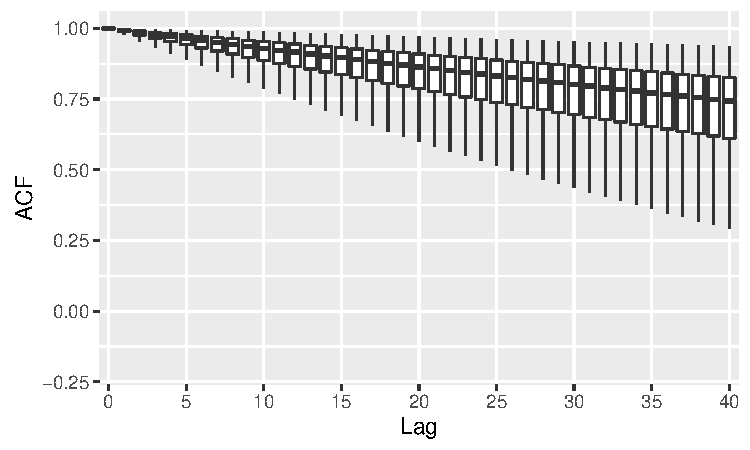
\includegraphics[width=0.3\linewidth]{binomial_random_acf_da}}%
%    \qquad
%    \subfigure[ACFs of the rate parameters $\theta_i$ using CDA.]{%
%      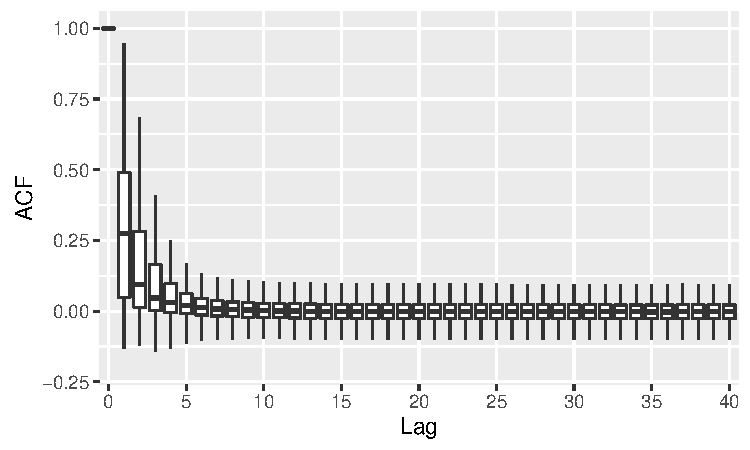
\includegraphics[width=0.3\linewidth]{binomial_random_acf_cda}}
%     \qquad
%    \subfigure[ACFs of the rate parameters $\theta_i$ using HMC.]{%
%      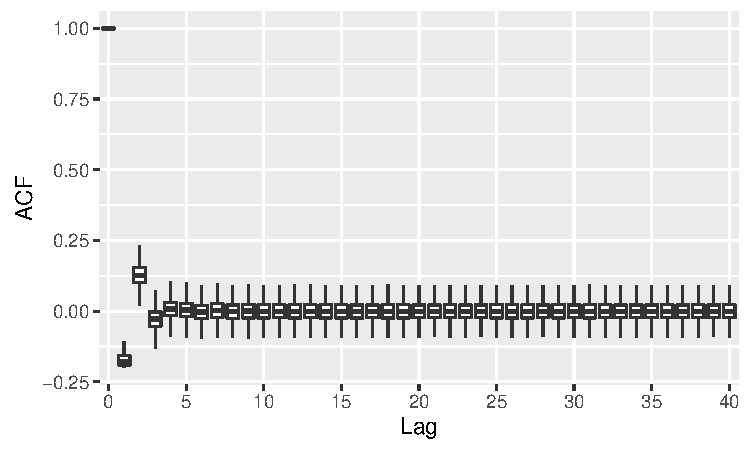
\includegraphics[width=0.3\linewidth]{binomial_random_acf_hmc}}
%  }
%\end{figure}
% 
% 
%\begin{table}[H]
%\small
%\centering
%\begin{tabular}{|l |r |r| r| r |} 
% \hline
%                          & DA & CDA & HMC\\
% [0.5ex]
%
% $ \sum \theta_i/n$      & -10.03 (-10.16, -9.87)& -12.05 (-12.09, -12.02) &  -12.06 (-12.09, -12.01)\\
% $ \sum \theta_i^2/n$      & 102.25 (98.92, 105.23)& 153.04 (152.06, 154.05) &  153.17 (152.02, 154.29)\\
%$\theta_0$          & -10.03 (-10.17, -9.87)& -12.05 (-12.09,-12.01) &  -12.06 (-12.10, -12.01)\\
%$\sigma^2$         & 1.60 (1.36, 1.82)&   7.70 (7.49, 7.88)  & 7.71 (7.51, 7.91)\\
%$T_{eff} / T$ & 0.0085 (0.0013 0.0188) & 0.5013 (0.1101,1.0084) & 0.8404 (0.5149, 1.2470)\\
%Avg Computing Time /  $T$  & 1.2 sec       & 1.2 sec        & 6 sec\\
%Avg Computing Time /  $T_{eff}$  & 140.4 sec       & 0.48 sec        & 1.3 sec\\
% \hline
%\end{tabular}
%\caption{Parameter estimates (with 95\% credible intervals) and computing speed (ratios among computing time, effective sample sizes $T_{eff}$ and total iterations $T$) of the DA, CDA and HMC in hierarchical binomial model. CDA provides parameter estimates as accurate as HMC, and is more computationally efficient than HMC.}
%\label{tab:binomial}
%\end{table}




\subsection{Poisson Log-Normal Model for Web Traffic Prediction}
As a second application, we apply CDA to an online browsing activity dataset obtained from a computational advertising company. The dataset contains a two-way  table of visit count by users who browsed one of $96$ websites belonging to clients of the computational advertising agency, and one of the  $n=59,792$ high-traffic sites during the same browsing session. We refer to visiting more than one site during the same session as co-browsing. For each of the client websites, it is of commercial interest to identify the high-traffic sites with relatively high co-browsing rates, so that ads can be more effectively placed. In computational advertising, it is also valuable to understand the co-browsing behavior and predict the traffic pattern of users. %We consider two models for these data.

%The co-browsing rate is commonly correlated with click-through rates for ads for the client site that are displayed on the high-traffic site. Therefore, the count of co-browsing is a useful indication of the click-through traffic. For any given client website, predicting the high traffic sites that could generate the most traffic is of high commercial interest. Therefore, 
We consider a Poisson regression model for co-browsing. We use the co-browsing count of a single client website as the outcome $y_i$ and the log of one plus the co-browsing count of the other $95$ websites as the predictors, i.e. $x_{ij}=\log (x^*_{ij}+1)$ for $i=1,\ldots ,59792$ and $j=1,\ldots ,95$, where $x^*$ is the raw co-browsing count for high-traffic site $i$ and client site $j$.  A Gaussian random effect is included to account for over-dispersion relative to the Poisson distribution, leading to a Poisson log-normal regression model: 
\be
 y_i \sim \Poi \left( \exp  (\xbeta + \tau_i )\right),  \quad \tau_i\stackrel{iid}{\sim} \No(\tau_0, \nu^2), \quad i=1\ldots n\\
 \beta \sim  \No(0, I \sigma_\beta^2), \quad \tau_0 \sim \No(0,\sigma_\tau^2) \quad \nu^2\sim \pi(\nu^2).
\ee
We assign a weakly informative prior for $\beta$ and $\tau_0$ with $ \sigma_\beta^2=\sigma_\tau^2=100$. For the over-dispersion parameter $\nu^2$, we assign a non-informative flat prior on $(0,\infty)$.

When $\beta$ and $\tau$ are sampled separately, the random effects $\tau = \{\tau_1,\ldots, \tau_n\}$ mix slowly. Instead, we sample $\beta$ and $\tau$ jointly. Letting $\tilde X$ be the $n \times (n+p)$ matrix given by $\tilde X = [ I_n\, X ]$, and $\eta_i=\xbeta + \tau_i$ the linear predictor, $\theta= \{\tau, \beta\}'$ can be sampled jointly in a block. An explanation of improved mixing with blocked sampling can be found in \cite{liu1994collapsed}.

We now focus on the mixing behavior of data augmentation. We first review data augmentation for the Poisson log-normal model. \cite{zhou2012lognormal} proposed to treat $\Poi(\eta_i)$ as the limit of the negative binomial $\NB\big(\lambda,{\eta_i}/{(\lambda+\eta_i)}\big)$ with $\lambda\rightarrow \infty$, and used moderate $\lambda=1,000$ for approximation. The limit relationship, omitting constants, is given by
\be
L(\eta_i;y_i)=\frac{ \exp(y_i \eta_i \} }{\exp\{\exp(\eta_i)\}} = \lim_{\lambda\rightarrow\infty}\frac{\exp(y_i \eta_i)}{\{1+ \exp(\eta_i )/\lambda\}^{\lambda }}.
\label{eq:pos_approx}
\ee

With finite $\lambda$ approximation, the posterior can be sampled using Polya-Gamma data augmentation
\be
z_i \mid \eta_i \sim  \PG ( & \lambda, \eta_i -\log \lambda)  \quad i=1\ldots n\\
\theta \mid z, y \sim  \No \bigg(  &  \Big(\tilde X' Z \tilde X+  \begin{bmatrix} 1/\nu^2 \cdot I_n & 0\\ 0 & 1/\sigma^2_{\beta}  \cdot I_p \end{bmatrix}\Big)^{-1} \\
& \bigg\{  \tilde X'  \big ( y - \lambda/2 + Z \log \lambda\big) +   \begin{bmatrix} \tau_0/\nu^2  1_n \\  0_p \end{bmatrix} \bigg\} , \\
& \Big(\tilde X' Z \tilde X+  \begin{bmatrix} 1/\nu^2 \cdot I_n & 0\\ 0 & 1/\sigma^2_{\beta}  \cdot I_p \end{bmatrix}\Big)^{-1} \bigg),
\ee
where $Z = \diag\{ z_1, \ldots,  z_n\}$, $1_n = \{1, \ldots, 1\}'$ and $0_p = \{0, \ldots 0\}'$.

However, this approximation-based data augmentation is inherently problematic.  For example, setting 
$\lambda = 1,000$ leads to large approximation error.  As in \eqref{eq:pos_approx}, the approximating denominator has $(1+\exp\left(\eta_i)/\lambda\right)^\lambda= \exp \{ \exp(\eta_i) + \bigO(\exp(2\eta_i)/\lambda) \}$; for moderately large $\eta_i \approx 10$, $\lambda$ needs to be at least $10^9$ to make $\exp(2\eta_i)/\lambda$ close to $0$. This large error cannot be corrected with an additional MH step, since the acceptance rate would be too low. On the other hand, it is not practical to use a large $\lambda$  in a Gibbs sampler, as it would create extremely large $z_i$  (associated with small conditional covariance for $\theta$), resulting in slow mixing.

We use CDA to circumvent this issue. We first choose a very large $\lambda$ ($10^9$) to control the approximation error, then use a small fractional $r_i$ multiplying to $\lambda$ for calibration. This leads to a proposal likelihood similar to the logistic CDA:
\be
L_{r,b}(\xtheta;y_i)=\frac{\exp(\eta_i   -\log \lambda +b_i)^{y_i}}{\{1+ \exp(\eta_i -\log \lambda +b_i)\}^{r_i\lambda  }},
\ee
with $r_i \ge (y_i-1)/\lambda + \epsilon$ for proper likelihood, and proposal update rule:
\be
z_i \sim  \PG ( & r_i\lambda, \eta_i -\log \lambda + b_i)  \quad i=1\ldots n\\
\theta^* \sim  \No \bigg(  &  \Big(\tilde X' Z \tilde X+  \begin{bmatrix} 1/\nu^2 \cdot I_n & 0\\ 0 & 1/\sigma^2_{\beta}  \cdot I_p \end{bmatrix}\Big)^{-1} 
\\&\Big\{  \tilde X'  \big( y - r\lambda/2 + Z \log (\lambda -b )\big) +   \begin{bmatrix} \tau_0/\nu^2  1_n \\  0_p \end{bmatrix} \Big\} , \\
& \Big(\tilde X' Z \tilde X+  \begin{bmatrix} 1/\nu^2 \cdot I_n & 0\\ 0 & 1/\sigma^2_{\beta}  \cdot I_p \end{bmatrix}\Big)^{-1} \bigg)
\ee
Letting $\eta_i^* = \tilde X \theta^*$, the proposal is accepted with probability (based on the Poisson density and the approximation $L_{r,b}(\xtheta;y_i)$):
\be
\min \bigg\{1 , \prod_i  \frac{ \exp \{ \exp (\eta_i)\}}{ \exp \{ \exp (\eta_i^*)\}} \frac {{\{1+ \exp(\eta_i^{*}  -\log \lambda +b_i)\}^{r_i\lambda }}}{{\{1+ \exp(\eta_i  -\log \lambda +b_i)\}^{r_i\lambda  }}} \bigg\}.
\ee
The tuning parameters are then optimized as described in Section~\ref{sec:tuning}, using
\begin{equation*}
	\begin{aligned}
    \tilde z_i(\theta) = &  \frac{\lambda r_i}{2|\eta_i -\log \lambda + b_i|} \tanh \left(\frac{|\eta_i -\log \lambda + b_i|}{2}\right) \quad i=1,\ldots,n, \\
    \tilde \theta^*(z) = &\Big(\tilde X' Z \tilde X+  \begin{bmatrix} 1/\nu^2 \cdot I_n & 0\\ 0 & 1/\sigma^2_{\beta}  \cdot I_p \end{bmatrix}\Big)^{-1} 
\\&\Big\{  \tilde X'  \big( y - r\lambda/2 + Z \log (\lambda -b )\big) +   \begin{bmatrix} \tau_0/\nu^2  1_n \\  0_p \end{bmatrix} \Big\}.
	\end{aligned}
\end{equation*}
After $\theta$ is updated, the other parameters can be sampled via  $\tau_0\sim \No\big( (n/ \nu^2 + 1/ \sigma^2_\tau)^{-1}$ $\sum_i \tau_i/\nu^2 , (n/ \nu^2 + 1/ \sigma^2_\tau)^{-1}  \big)$ and $\nu^2 \sim \IG ( n/2-1, \sum_i (\tau_i-\tau_0)^2 /2)$.

We ran the ordinary DA algorithm with $\lambda=1,000$, CDA with $\lambda=10^9$ and Hamiltonian Monte Carlo with No-U-Turn sampler under the default tuning setting (as implemented in \texttt{STAN 2.17}). All algorithms are initialized at the MAP. We ran DA for $200,000$ steps, CDA for $2,000$ steps and HMC for $20,000$ steps so that they have approximately the same effective sample size. For CDA, we used the first $1,000$ steps for adapting $r$ and $b$. Figure~\ref{data_poisson} shows empirical autocorrelations for DA, CDA and HMC. Even with small $\lambda = 1,000$ in DA, all of the parameters mix poorly; HMC seemed to be affected by the presence of random effects, and most of parameters remain highly correlated within $40$ lags; CDA substantially improves the mixing. Table~\ref{table:Poisson} compares all three algorithms. CDA has the most efficient computing time per effective sample, and is about $30-300$ times more efficient than the other two algorithms.
\begin{figure}[H]
  {%
    \subfigure[Autocorrelation of the parameters from DA.]{%
      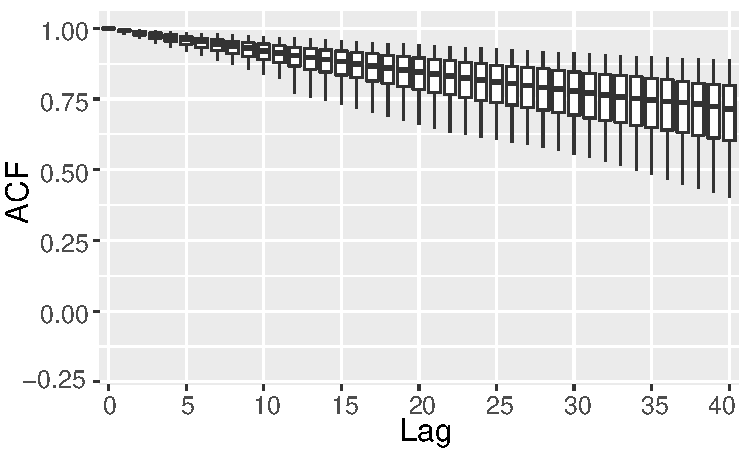
\includegraphics[width=0.32\linewidth]{poisson_acf_da}}%
    \quad
    \subfigure[Autocorrelation of the parameters from CDA.]{%
      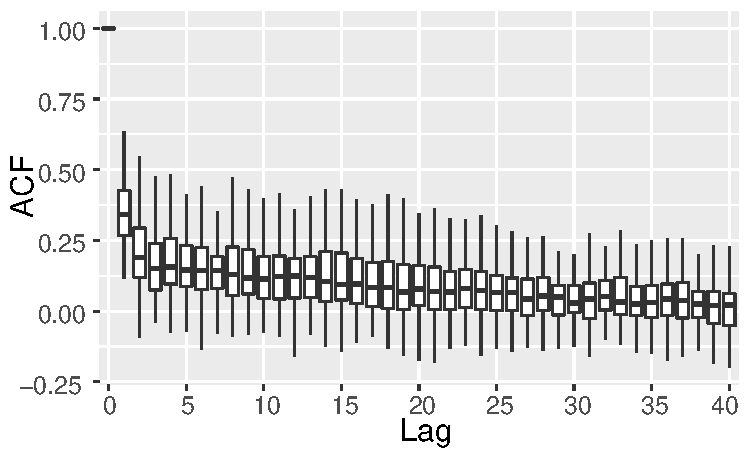
\includegraphics[width=0.32\linewidth]{poisson_acf_cda}}
      \centering
    \subfigure[Autocorrelation of the parameters from HMC.]{%
      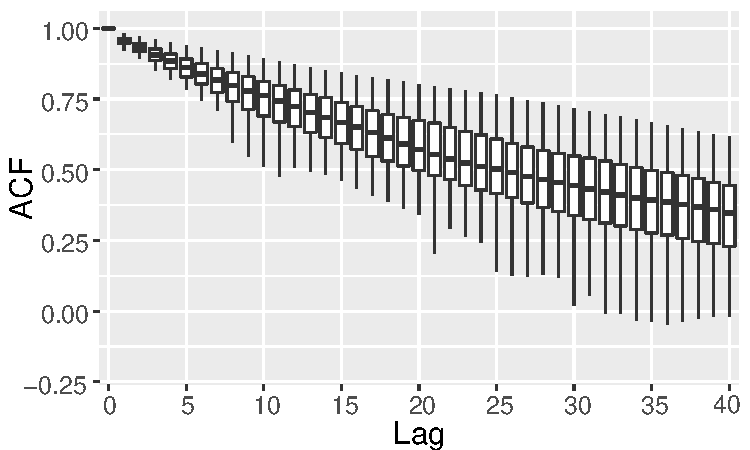
\includegraphics[width=0.32\linewidth]{poisson_acf_hmc}}
  }
    {\caption{CDA significantly improves the mixing of the parameters in the Poisson log-normal. \label{data_poisson}}}
\end{figure}
 
To evaluate predictive performance, we use another co-browsing count table for the same high traffic and client sites, collected during a different time period. We use the high traffic co-browsing count $x_{ij}^{\dagger*}$ and their log transform 
$x^\dagger_{ij} = \log(   x_{ij}^{\dagger*} +1 )$ for the  $j = 1,\ldots,95$ clients to predict the count for the client of interest $y_i^\dagger$, over the high traffic site $i=1,\ldots, 59792$. We predict using $\hat y_i^\dagger= \bb E_{ \beta, \tau \mid y,x}   y_{i}^\dagger =\bb E_{ \beta, \tau \mid y,x}\exp(  x_{i}^\dagger\beta + \tau_i)$ on the client site. The expectation is approximated using the MCMC sample path for $\beta, \tau \mid y,x$ obtained using training set $\{y,x\}$, as discussed above. Cross-validation root-mean-squared error $\big(\sum_i(\hat y_i^\dagger - y_i^\dagger)^2/n\big)^{1/2}$ between the prediction and actual count $ y_i^\dagger$'s is computed. As shown in Table~\ref{table:Poisson}, slow mixing in DA and HMC cause poor estimation of the parameters and high prediction error, while CDA has significantly lower error. 
\begin{table}[H]
\footnotesize
\centering
\begin{tabular}{|l |r |r| r| r |} 
 \hline
                          & DA & CDA & HMC\\
 [0.5ex]
$\sum \beta_j / 95$         & 0.072 (0.071, 0.075)&  -0.041 (-0.042, -0.038)  & -0.010 (-0.042, -0.037) \\
$\sum \beta_j^2 / 95$         & 0.0034 (0.0033, 0.0035)&  0.231 (0.219 0.244)  & 0.232 (0.216 0.244)   \\
$\sum\tau_i/n$         & -0.405 (-0.642, -0.155)&  -1.292 (-2.351, -0.446)  &  -1.297 (-2.354, -0.451)  \\
$\sum\tau_i^2/n$         & 1.126 (0.968, 1.339)&  3.608 (0.696, 7.928)  & 3.589 (0.678, 8.011)  \\
% RMSE                              & 30.83        & 4.03          & 7.38\\
Prediction RMSE                           & 33.21        & 8.52          & 13.18\\
$T_{eff} / T$ & 0.0037 (0.0011 0.0096) & 0.3348 (0.0279, 0.699) &  0.0173 (0.0065, 0.0655) \\
Avg Comp. Time /  $T$  & 1.3 sec       & 1.3 sec        & 56 sec\\
Avg Comp. Time /  $T_{eff}$  & 346.4 sec       & 11.5 sec        & 3240.6 sec\\
 \hline
\end{tabular}
\caption{Parameter estimates, prediction error and computing speed of the DA, CDA and HMC in Poisson regression model.}
\label{table:Poisson}
\end{table}

\section{Discussion}
Data augmentation (DA) is a technique routinely used to enable implementation of simple Gibbs samplers, avoiding the need for expensive and complex tuning of Metropolis-Hastings algorithms.
Despite the convenience, DA mixes slowly when the conditional posterior variance given the augmented data is substantially smaller than the marginal variance.  When the data sample size is massive, this problem arises when the rates of convergence of the augmented and marginal posterior differ. There is a rich literature on strategies for improving mixing rates of Gibbs samplers, with centered or non-centered re-parameterizations \citep{papaspiliopoulos2007general} and parameter-expansion \citep{liu1999parameter} leading to some improvements.  However, existing approaches {do not} solve large sample mixing problems because they do not address the fundamental rate mismatch issue.

To tackle this problem, we propose to calibrate data augmentation by directly adjusting the conditional variance (which is associated with step size).  CDA adds a small cost for likelihood evaluation, which is often negligible when compared to the random number generation required at each iteration of DA. In this article, we demonstrate that calibration is generally applicable when $\theta \mid z$ belongs to a location-scale family. We expect it to be also useful outside of location-scale families, but have not pursued that here.

As both CDA and HMC involve MH steps, we draw some further comparison between the two. Both methods rely on finding a good proposal by searching a region far from the current state. One key difference lies in the computing efficiency. Although HMC is more generally applicable beyond data augmentation, it is computationally intensive since Hamiltonian dynamics often requires multiple numeric steps. CDA only requires one step of calibrated Gibbs sampling, which is often much more efficient, leveraging on existing data augmentation algorithms. The idea of using an auxiliary Gibbs chain to generate MH proposals seems generally promising \citep{tran2016adaptive}, yet has received little attention in the literature.

{In this work, we focused on cases when the sample size  $n$ is large, with the parameter dimension $p$ moderate. One limitation of CDA-MH is that when $p$ grows, in order to maintain a reasonable acceptance rate, the range to increase the conditional variance has to decrease. This is a common problem for general MH algorithms. Therefore, solutions to high dimensionality require further study.}

%\bigskip
%\begin{center}
%{\large\bf SUPPLEMENTARY MATERIAL}
%\end{center}

\appendix

\section{Proof of Remark \ref{rem:accrat}}
\begin{proof}
Since $q_{r,b}(\theta;\theta')$ is the $\theta$ marginal of a Gibbs transition kernel, and Gibbs is reversible on its margins, we have
\be
q(\theta;\theta^*) \Pi_{r,b}(\theta^*) = q(\theta^*;\theta) \Pi_{r,b}(\theta),
\ee 
and so
\be
\frac{L(\theta^*;y) \Pi^0(\theta^*) q(\theta;\theta^*)}{L(\theta;y) \Pi^0(\theta) q(\theta^*;\theta)} &= \frac{L(\theta^*;y) \Pi^0(\theta^*) L_{r,b}(\theta;y) \Pi^0(\theta) }{L(\theta;y) \Pi^0(\theta) L_{r,b}(\theta^*;y) \Pi^0(\theta^*)} \\
&= \frac{L(\theta^*;y)L_{r,b}(\theta;y)}{L(\theta;y) L_{r,b}(\theta^*;y)}.
\ee
\end{proof}

\section{Proof of Remark \ref{rem:ergodic}}
\begin{proof}
For any $r,b$, the conditionals $\Pi_{r,b}(z \mid \theta)$ and $\Pi_{r,b}(\theta \mid z)$ are well-defined for all $z \in \mc Z, \theta \in \Theta$, and therefore the Gibbs transition kernel $K_{r,b}((\theta,z);\cdot)$ and corresponding marginal kernels $Q_{r,b}(\theta;\cdot)$ are well-defined. Moreover, for any $(z,\theta) \in \mc Z \times \Theta$, we have $\bb P[(\theta',z') \in A \mid (\theta,z)] > 0$ by assumption. Thus $K_{r,b}$ is aperiodic and $\Pi_{r,b}$-irreducible (see the discussion following Corollary 1 in \cite{roberts1994simple}).

$Q_{r,b}(\theta';\theta)$ is aperiodic and $\Pi_{r,b}(\theta)$-irreducible, since it is the $\theta$ marginal transition kernel induced by $K_{r,b}((\theta,z);\cdot)$. Thus, it is also $\Pi(\theta)$-irreducible so long as $\Pi \gg \Pi_{r,b}$, where for two measure $\mu,\nu$, $\mu \gg \nu$ indicates absolute continuity. Since $\Pi, \Pi_{r,b}$ have densities with respect to Lebesgue measure, $\Pi_{r,b}$-irreducibility implies $\Pi$ irreducibility. Moreover, $q(\theta;\theta') > 0$ for all $\theta \in \Theta$. Thus, by Theorem 3 of \cite{roberts1994simple}, CDA MH is $\Pi$-irreducible and aperiodic. 
\end{proof}




\section{Toy example: Hierarchical Normal \label{gaussian_example}}

To demonstrate the effects of $r,b$, we use a toy example commonly used in the data augmentation literature \citep{liu1999parameter}. Consider a marginal Normal model
\begin{equation*}
	\begin{aligned}
    y_i \sim \No(\theta, \sigma^2+1) \qquad i=1,\ldots,n
	\end{aligned}
\end{equation*}
with $\sigma^2$ known and improper prior $\pi(\theta)\propto 1$. This can be considered as a hierarchical model

\begin{equation}
\label{hier_normal_model}
	\begin{aligned}
    y_i \sim \No(z_i, \sigma^2), \quad z_i\sim \No(\theta,1), \qquad i=1,\ldots,n,
	\end{aligned}
\end{equation}
where $z=\{z_1,\ldots,z_n\}$ are augmented data. The standard data augmentation algorithm has the update rule

\begin{equation*}
	\begin{aligned}
    z_i \mid y,\theta&\sim \No \left(\frac{y_i\sigma^{-2}+\theta}{\sigma^{-2}+1}, \frac{1}{\sigma^{-2}+1} \right) \qquad i=1,\ldots,n \\
    \theta \mid z & \sim \No({n}^{-1}{\sum_i z_i}, {n}^{-1}).
	\end{aligned}
\end{equation*}

Thanks to the simple form, it is straightforward to compute the marginal variance of $\theta$, $\mbox{var}(\theta\mid y) = {n}^{-1}(1+\sigma^2)$. Clearly, this is larger than the conditional variance  $\mathbb{E}_z\mbox{var}(\theta'\mid z)=n^{-1}$, when $\sigma^2$ is large.

To be able to adjust the conditional variance, we consider an alternative hierarchical model

\begin{equation*}
	\begin{aligned}
    y_i \sim \No(z_i, \sigma^2), \quad z_i\sim \No(\theta+b_0,r_0), \qquad i=1,\ldots,n,
	\end{aligned}
\end{equation*}
with update rule
\begin{equation}
\label{hier_model_proposal}
	\begin{aligned}
    z_i \mid y,\theta&\sim \No \left(\frac{y_i\sigma^{-2}+(\theta+b_0)r_0^{-1}}{\sigma^{-2}+r_0^{-1}}, \frac{1}{\sigma^{-2}+r_0^{-1}} \right) \qquad i=1,\ldots,n \\
    \theta^* \mid z & \sim \No({n}^{-1}{\sum_i z_i}-b_0 , {n}^{-1}r_0).
	\end{aligned}
\end{equation}
To  correct the deviation caused by the alternative model, we treat $\theta^*$ as a proposal to the target model \eqref{hier_normal_model}, using M-H as in Remark \ref{rem:accrat} with $L_{r,b}(\theta;y)= (r_0 + \sigma^2)^{-1/2}\phi[ (r_0 + \sigma^2)^{-1/2}(y_i - \theta - b_0)]$ and $\phi$ the standard normal density. We can choose $r_0$ so that the proposal variance equals to the target marginal variance $\mbox{var}_{r,b}(\theta'\mid z) = \mbox{var}(\theta\mid y) $; this yields

\begin{equation*}
	\begin{aligned}
    r_0=1+\sigma^2.
	\end{aligned}
\end{equation*}

Note the proposal mean has

\begin{equation*}
	\begin{aligned}
        \mathbb{E} (\theta^* \mid \theta)=\mathbb{E}_{z\mid \theta} \mathbb{E}_{\theta^*\mid z} (\theta^*\mid z)= \theta + {\frac{n^{-1}\sum_i y_ir_0 }{\sigma^{2}+r_0}- \frac{(b_0 + \theta)r_0}{\sigma^{2}+r_0} }
	\end{aligned}
\end{equation*}
Intuitively, one way to improve the acceptance rate is to have the proposal centered at the current $\theta$ in the high posterior density region. That is, $  \mathbb{E} (\theta^*\mid \theta)\approx \theta$ for $\theta$ near the MAP $\hat\theta = n^{-1}\sum_i y_i$. This yields one choice for $b_0$

\begin{equation*}
	\begin{aligned}
    \frac{n^{-1}\sum_i y_ir_0 }{\sigma^{2}+r_0}- \frac{(b_0 + \hat\theta)r_0}{\sigma^{2}+r_0} =0 \qquad \Rightarrow b_0=0
	\end{aligned}
\end{equation*}

We use $\sigma^2=100$, $\theta=1$ to simulate  $n=1000$ data. Figure~\ref{plot_hierarchical_normal} compares the mixing performance, in terms of traceplots and autocorrelation plots (ACF) for the original DA and calibrated DA. Each algorithm was initiated at the MAP $\hat\theta= n^{-1}\sum_iy_i$. CDA significantly improves the mixing performance, with acceptance rate approximately $0.9$.

\begin{figure}[H]
  {%
    \subfigure[Traceplot for DA and CDA.]{
      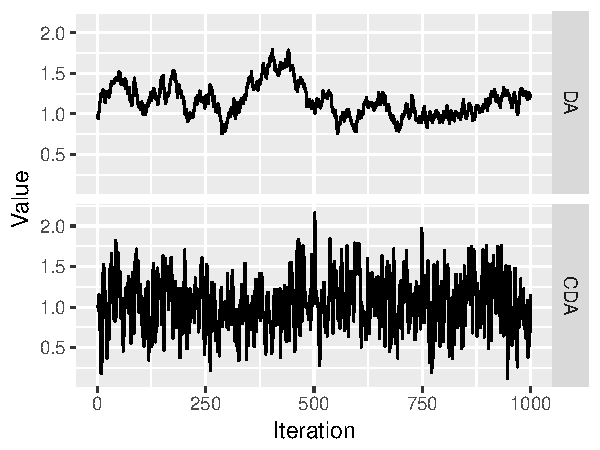
\includegraphics[width=0.49\linewidth]{traceplot_hier_normal}}%
%    \qquad
    \subfigure[ACF for DA and CDA.]{
      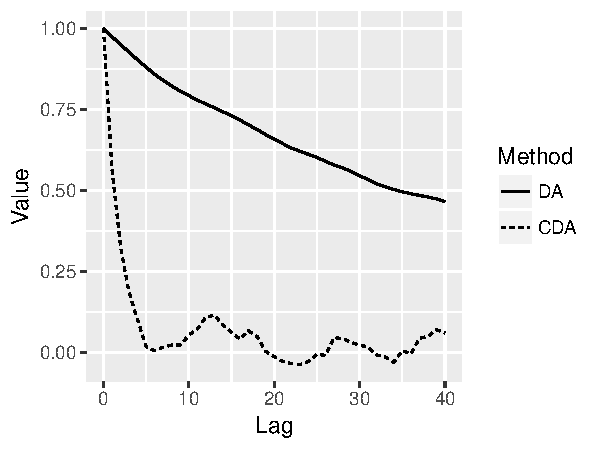
\includegraphics[width=0.49\linewidth]{acf_hier_normal}}
  }
    {\caption{Trace and autocorrelation plots for DA and CDA in hierarchical normal model.\label{plot_hierarchical_normal}
}}
\end{figure}



Note in this special example, instead of relying on $\mbox{var}_{r,b}(\theta^*\mid z)$, one could directly adjust $ \mbox{var}_{r,b}(\theta^*\mid \theta)=[r_0^2 + 2r_0 \sigma^2]/[n(r_0+\sigma_0^2)]$ to match $ \mbox{var}(\theta\mid y)$. However, in general non-Gaussian cases, $\mbox{var}_{r,b}(\theta^*\mid \theta)$ is intractable, so we expect adjusting $\mbox{var}(\theta^*\mid z)$ to be more useful.


%
%{
%\subsection{Diagnostics of Adaptation}
%}
%We adapt the tuning parameters $(r,b)$ by locally minimizing difference between two Fisher information matrices and
% optimizing acceptance rate near 
% $\hat\theta_{MAP}$ during adaptation. Updating $b$  as a function
% of $\theta$ yields $L_{r,b}(\theta;y)=L(\theta;y)$ exactly;  after adaptation,
%for  fixed
% $(r,b)$, $L_{r,b}(\theta;y)$ is close to $L(\theta;y)$ for $\theta$ in the neighborhood
% around $\hat\theta_{MAP}$. To show this empirically, consider the
% probit Bernoulli regression example. As the $L(\theta;y)$ and $L_{r,b}(\theta;y)$
% are parameterized by $\Phi(x_i\beta)$ and $\Phi(({x_i\beta+b_i})/{\sqrt{r_i}})$, Figure~\ref{probitAdaptDiag}(a) compares the posterior values of $x_i\beta$ against
%$({x_i\beta+b_i})/{\sqrt{r_i}}$. Clearly, the two are very close with a
%RMSE of $0.23$.
%Figure~\ref{probitAdaptDiag}(b) shows the trace of the adaptation of $r$
%during
%the initial $400$ iterations;
%$r$ quickly rises from $1$ to the roughly  appropriate scale during the
%initial $50$ steps. The values of $(r,b)$ are fixed afterwards to ensure
%ergodicity.
%
%\begin{figure}[H]
%  {\caption { Diagnostics plot of the adaptation for probit regression. \label{probitAdaptDiag}}}
%  {%
%    \subfigure[Posterior sample of $x_i\beta$ and its corresponding transform
%$({x_i\beta+b_i})/{\sqrt{r_i}}$  in probit CDA.]{%
%      \includegraphics[width=0.45\linewidth]{adaptDiag}}%
%    \qquad
%    \subfigure[Trace of the adaptation of r, shown on log scale.]{%
%      \includegraphics[width=0.45\linewidth]{adaptTraceR}}
%  }
%\end{figure}
% \subsection{Numeric Distances between MH Proposal and Posterior}
% \label{wass2-proposal}

% To empirically demonstrate that CDA proposal is closer to the target density, we compute the numeric Wasserstein$-2$ distances between proposal and posterior in probit regression under different dimension $p$. To obtain proposal samples from $Q(\theta^*;\theta)$, we fixed $\theta=\hat\theta$ and generate $1,000$ independent samples. Wasserstein$-2$ distance is then computed between those proposals and $1,000$ posterior samples obtained from MCMC. We repeated experiments using probit-CDA, Gaussian random walk and uniform random walk with the same variance $(X^T\hat RX)^{-1}$. As shown below, the CDA-proposal has the lowest distance to the posterior under all $p=1,\ldots,30$.

% \begin{figure}[H]
%   {\caption { Numeric Wasserstein$-2$ distances between proposal and posterior in probit regression under different dimension $p$. \label{probitAdaptDiag}}}
% {
%       \includegraphics[width=0.8\linewidth]{w2_distance_proposal.pdf}}
% \end{figure}



{
\section{Calibrated  Polya-Gamma Algorithm with Sub-sampling}
}
Adapting based on \cite{johndrow2015approximations}, we first randomly sample
a subset of indices $V$ of size $|V|$. This algorithm  generates proposals from

\be
V & = V_1\cup V_0,\quad V_1= \{i\in\{1,\ldots,n\}: y_i=1\}, \quad V_0  \sim \text{Subset}(|V|,\{i\in\{1,\ldots,n\}: y_i=0\})
\\ z_i &\sim {\PG}(k_{i}r_i, |\xtheta+b_i|) \quad i\in V,\\
\theta^* &\sim \No \left(  (X_V' Z_{V} X_V)^{-1}  X_V'  (y_V -k_{V}r_V/2- Z_Vb_V) ,  (X_V' Z_V X_V)^{-1}  \right),
\ee
where subscript $._V$ indicates the sub-matrix or sub-vector corresponding
to the sub-sample; $k_i=1$ if $y_i=1$, and
$k_i=({n-|V_1|})/{|V_0|}$. We accept $\theta^*$ in an MH step using calibrated
likelihood 
$$L_{r,b}(\theta;y) = \prod_{i\in V_1}\frac{\exp(x_i\theta+b_i)}{\{ 1+\exp(x_i\theta+b_i)\}^{r_i}}  (\prod_{i\in V_0}\frac{1}{\{ 1+\exp(x_i\theta+b_i)\}^{r_i}}
)^{\frac{n-|V_1|}{|V_0|}}
,$$
with target approximate likelihood  $L_{1,0}(\theta;y)$.
%Using Fisher information, the  parameters are adapted initially for $200$
% steps, via 
% \be r_{i} & =\frac{\exp(x_i\theta)}{ \{1+\exp(x_i\theta)\} ^2} / \left (   \frac{1}{2 |x_i\theta+b_{i}|} \tanh\frac{|x_i\theta+b_{i}|}{2} \right) \vee \big ( ( y_i-1)/k_{i} + \epsilon \big)\\
%b_{i} & =\log[  \{1+\exp(x_i\theta+b_{i})\}^{1/r_{i}} -1] - x_i\theta.\ee


\section{Proof of Theorem 1}
\begin{proof}
Let $Q$ be the proposal kernel for CDA-MH, which is identically the transition kernel for CDA-Gibbs, and let $\mc P$ be the Markov transition semigroup of CDA-MH.

 Both have densities with respect to Lebesgue measure given by
 \be
q(\theta,\theta') &= \int_{\mathcal{Z}}f_{r,b}(\theta' \mid z,y) \pi_{r,b}(z \mid \theta, y ) d z \\
p(\theta,\theta') &= \alpha(\theta,\theta') q(\theta,\theta') + \delta_\theta(\theta') \left(1-\int \alpha(\theta,\tilde \theta) q(\theta,\tilde \theta) d \tilde \theta \right),
\ee
respectively.

We seek a constant $c>0$ and a density $g$ such that
\be
\inf_{\theta \in \Theta} p(\theta,\theta') > c g(\theta')
\ee
% 
% \begin{equation*}
% 	\begin{aligned}
%   &  K(\theta' \mid \theta) = \int_{\mathcal{Z}}\pi_{r,b}(\theta'\mid z,y) \pi_{r,b}(z \mid \theta, y ) d z\\
%   &  K(\theta^* \mid \theta) = \bigg[\alpha(\theta,\theta') \delta_{\theta'} (\theta^*)+ (1-\alpha(\theta,\theta'))\delta_\theta (\theta^*)\bigg] K(\theta'\mid \theta) 
% 	\end{aligned}
% \end{equation*}
% where $\alpha(\theta,\theta')$ is the acceptance probability.

We proceed in the following steps:

\begin{enumerate}
	\item Show that there exists a constant $c_1 > 0$ and a density $g$ such that $\int_{\Theta} g(\theta) d\theta = 1$ for which
	\be
	\inf_{\theta \in \Theta} q(\theta,\theta') \ge c_1 g(\theta');
	\ee
	conclude that CDA-Gibbs is uniformly ergodic.
	\item Show that there exists $S \subset \Theta$ and a constant $c_2 > 0$ such that 
	\be
	\inf_{\theta \in \Theta, \theta' \in S} \alpha(\theta,\theta') > c_2.
	\ee    
	\item Combine 1 and 2 to show $p(\theta,\theta') \ge \kappa g_S(\theta')$, where $\kappa= c_1c_2c_3$ with 
	\be
	c_3= \int_S g(\theta) d\theta, \quad g_S(\theta) = c_3^{-1} g(\theta) \1\{\theta \in S\}  
	\ee
	the restriction of $g$ to $S$. Conclude that CDA-MH is uniformly ergodic with spectral gap $\kappa$.
	\item Find values ${(r_0,b_0,S_0)}$ of the tuning parameters $r,b,S$ so that $\kappa$ goes to zero slowly as $n \to \infty$. 
    %has $\kappa(r_0,b_0,S_0) \gg c_1(1,0,\Theta)$ as $n$ increases, that is, $\lim_{n\to \infty} c_1(1,0,\Theta) /\kappa(r_0,b_0,S_0) =0$.
\end{enumerate}
%where $c_1(1,0,\Theta)$ is the convergence rate for DA-Gibbs algorithm. 

\textbf{1. Show that $q(\theta,\theta') \ge c_1 g(\theta')$.}
First we bound $\pi_{r,b}(\theta' \mid z)$ by a constant times a function depending on $z$
\be
 \pi_{r,b} & (\theta'\mid z) = (2\pi)^{-1/2} { ( z + 1/\sigma^2)}^{1/2} \exp\bigg[ -\frac{1}{2} (\theta'-m) ( z + 1/\sigma^2)  (\theta'-m)\bigg] \\
= & (2\pi)^{-1/2} { (z + 1/\sigma^2)}^{1/2} \exp\bigg[ -\frac{1}{2} 
\bigg\{
(\theta'+b)(z+ 1/\sigma^2)(\theta' +b) -2 a(\theta'+b) + \frac{a^2}{z+ 1/\sigma^2}
\bigg\}
\bigg] \\
> & (2\pi)^{-1/2} { ( 1/\sigma^2)}^{1/2} \exp\bigg[ -\frac{1}{2} 
\bigg\{
(\theta'+b)(z+ 1/\sigma^2)(\theta' +b) -2 a(\theta'+b) + \frac{a^2}{1/\sigma^2}
\bigg\}
\bigg] \\
= & (2\pi)^{-1/2} {\sigma^{-1}} \exp\bigg[ -\frac{1}{2} 
\bigg\{
(\theta'+b)^2/\sigma^2  -2 a(\theta'+b) + {a^2 {\sigma^2}} 
\bigg\}
\bigg] \exp\bigg[ -\frac{1}{2} 
\bigg\{ (\theta'+b)^2 z 		\bigg\}
\bigg] \\\label{eq:LB1}
\ee
in which the inequality holds since $z>0$.

Using the Laplace transform of $\omega \sim \text{PG}(\alpha,\beta)$
\be    
\bb{E}[ \exp(-\omega t )] = \frac{\cosh^\alpha(\beta/2)}{\cosh^\alpha(\sqrt{(\beta^2/2+t)/2})},
\ee
we proceed to bound the expectation of \eqref{eq:LB1} with respect to $z$
\be
\int_{0}^{\infty} &\exp\bigg[ -\frac{1}{2} 
\bigg\{ (\theta'+b)^2 z 		\bigg\}
\bigg]  \pi_{r,b}(z \mid \theta ) d {z}  = 
{\cosh^{nr} (\frac{|\theta+b|}{2})}{\cosh^{-nr} (\frac{\sqrt{((\theta+b)^2+ (\theta'+b)^2)}}{2})}\\
& \ge 	 {\cosh^{nr} (\frac{|\theta+b|}{2})}{\cosh^{-nr} (\frac{{(|\theta+b|+ |\theta'+b|)}}{2})}\\
& \ge 	 2^{-nr}{\cosh^{nr} (\frac{|\theta+b|}{2})}{{\cosh^{-nr} (\frac{|\theta+b|}{2})}}{{\cosh^{-nr} (\frac{|\theta'+b|}{2})}}\\
& = 2^{-nr}\cosh^{-nr} (\frac{|\theta'+b|}{2}) \\
& \ge 2^{-nr} \exp \bigg [- \frac{nr|\theta'+b|}{2} \bigg ] \\
& \ge 2^{-nr} \exp \bigg [ - \frac{nr [ (\theta'+ b)^2+1]}{4} \bigg ]
\ee
where the first inequality uses $a^2+b^2 \le (|a|+|b|)^2$; the second uses Lemma 3.2 of Choi and Hobert  (2013); the third uses the property of $\cosh$; and the fourth uses $|a| \le (1+a^2)/2$. We combine to obtain $q(\theta,\theta') > c_1 g(\theta')$, viz 
\be
q&(\theta,\theta')  =
\int_{0}^{\infty} \pi_{r,b}(\theta' \mid z ,y_{1:n}) \pi_{r,b}(z \mid  \theta , y_{1:n}) d {z} \\
>&   (2\pi)^{-1/2} {\sigma^{-1}} \exp\bigg[ -\frac{1}{2} 
\bigg\{
(\theta'+b)^2/\sigma^2  -2 a(\theta'+b) + {a^2 {\sigma^2}} 
\bigg\}
\bigg]2^{-nr} \exp \bigg [ - \frac{nr [ (\theta'+ b)^2+1]}{4} \bigg ]\\
= & 
(2\pi)^{-1/2}  {\sigma^{-1}} 2^{-nr} \exp\bigg[ -\frac{1}{2} 
\bigg\{
(\theta'+b)^2 ( \frac{1}{\sigma^2} + \frac{nr}{2})  -2 a(\theta'+b)  
\bigg\}
\bigg] \exp \bigg [ - \frac{nr }{4} - \frac{a^2 \sigma^2  }{2} \bigg ]
\\
 %complete square
 = & {\sigma^{-1}} 2^{-nr}  (\frac{1}{\sigma^2}+\frac{nr}{2})^{-1/2} 
 \exp \bigg [ - \frac{nr }{4} - \frac{a^2 \sigma^2  }{2} \bigg ] 
 \exp \bigg [ \frac{1 }{2} a^2  (\frac{1}{\sigma^2}+\frac{nr}{2})^{-1}  \bigg ]
 \\
 &  (2\pi)^{-1/2} (\frac{1}{\sigma^2}+\frac{nr}{2})^{1/2} \exp\bigg[ -\frac{1}{2} 
 \bigg (\theta^{\prime}+b -(\frac{1}{\sigma^2}+\frac{nr}{2})^{-1} a\bigg)^2  (\frac{1}{\sigma^2}+\frac{nr}{2}) 	\bigg] \\
 = &c_1 g(\theta')
 \ee
 where
 \be
 c_1 &=  {\sigma^{-1}} 2^{-nr}  (\frac{1}{\sigma^2}+\frac{nr}{2})^{-1/2} 
 \exp \bigg [ - \frac{nr }{4} - \frac{a^2 \sigma^2  }{2} \bigg ] 
 \exp \bigg [ \frac{1 }{2} a^2  (\frac{1}{\sigma^2}+\frac{nr}{2})^{-1}  \bigg ] \\
 g(\theta') &=\No\bigg[\theta' \mid  (\frac{1}{\sigma^2}+\frac{nr}{2})^{-1} a -b, (\frac{1}{\sigma^2}+\frac{nr}{2})^{-1}\bigg].
 \ee
 This completes the first part.

%%%%%%%%%%%%%%%%%%%%%%%%%%%%%%
\textbf{2. Show that $\inf_{\theta \in \Theta, \theta' \in S} \alpha(\theta,\theta')> c_2$ for some set $S$.}

The acceptance ratio is
\be
\alpha(\theta,\theta') = \min \bigg( { \bigg[\frac{\alpha_0(\theta')}{\alpha_0(\theta)}\bigg]^n, 1 \bigg), \qquad 
\alpha_0(x) = 
\frac{\{1+\exp(x+b)\}^{r} } {1+\exp(x)}}
\ee

Differentiating with respect to $x$ we obtain
\be
\frac{\partial \alpha_0(x)}{\partial x}=&   \frac{e^x \left(e^{b+x}+1\right)^{r-1} \left( (r-1) e^b e^x+e^b r-1\right)}{\left(e^x+1\right)^2},\\
\ee
Assuming that $r < 1$ and $e^b r > 1$, since
\be
\frac{e^x \left(e^{b+x}+1\right)^{r-1}}{\left(e^x+1\right)^2}>0 
\ee
and there is only one root on $(-\infty,\infty)$ for
\be
(r-1) e^b e^x+e^b r-1 &= 0 \quad \Longrightarrow \quad x= \log(\frac{ e^b r -1}{ 1-r}) - b \equiv \hat \theta \\
(r-1) e^b e^x+e^b r-1 &<0 \quad \Longrightarrow \quad x > \hat \theta \\
(r-1) e^b e^x+e^b r-1 &>0 \quad \Longrightarrow \quad x < \hat \theta 
\ee
%which we denote by $\hat\theta$ from now on. Note ${\partial \alpha_0(x)}/{\partial x}>0$ when $x<\hat\theta$, $\alpha_0(x)$ monotonically increasing;  and ${\partial \alpha_0(x)}/{\partial x}<0$ when $x>\hat\theta$, $\alpha_0(x)$ monotonically decreasing. 
Therefore, $\hat \theta$ is the unique mode of $\alpha_0$, and $\alpha_0$ is (1) monotonically increasing for $x < \hat \theta$ and monotonically decreasing for $x > \hat \theta$.
%$\alpha(\hat\theta) = \sup_{x \in \mathbb{R}} \alpha_0(x)$ and $\hat \theta$ is the unique mode of $\alpha_0$.

For convenience, we write $b = -\log(r) + \xi$ with $\xi> 0$, so that $1+\exp(\hat\theta+b)= (e^{\xi}-r)/(1-r)$. Now set $S=(s_1,s_2)$. We now show that $\alpha(\theta,\theta') > c_2$ for $\theta' \in S$. We proceed in two cases.

\begin{enumerate}
	\item \textbf{Case 1}: $\theta\le \hat\theta$. We have three subcases
	\begin{enumerate}
		\item If $\theta < \theta' \le \hat\theta$, then $\alpha_0(\theta')\ge \alpha_0(\theta)$, $\alpha(\theta,\theta')=1$.

		\item If $s_1<\theta' \le \theta \le \hat\theta$ then

		\be
		\alpha(\theta,\theta')=  &\bigg(\frac{1+\exp(\theta)}{1+\exp(\theta')} \bigg)^n
		\bigg(\frac{1+\exp(\theta'+b)}{1+\exp(\theta+b)} \bigg)^{rn} \\
		\ge & 1 \times\quad \bigg(\frac{1}{1+\exp(\hat\theta+b)} \bigg)^{rn} = \bigg(\frac{1-r}{e^{\xi}-r} \bigg)^{rn}
		\ee

		\item If $\theta\le \hat\theta<\theta'<s_2$,

		\be
		\alpha(\theta,\theta')=  &\bigg(\frac{1+\exp(\theta)}{1+\exp(\theta')} \bigg)^n
		\bigg(\frac{1+\exp(\theta'+b)}{1+\exp(\theta+b)} \bigg)^{rn}\\
		\ge & \bigg(\frac{1}{1+\exp(\theta')} \bigg)^n \times 1 \ge \bigg(\frac{1}{1+\exp(s_2)} \bigg)^n
		\ee
		where we used that $\theta'>\theta$ so the second term is bounded below by 1, and that $1+e^\theta > 1$. 
	If $s_2\le \hat\theta$, then $\theta'<\hat\theta$, we only need to consider the condition (a) and (b).
	\end{enumerate}


	
	\item \textbf{Case 2:} $\theta > \hat\theta$,
	\begin{enumerate}
		\item If $\hat\theta<\theta' \le \theta$, then $\alpha_0(\theta')\ge \alpha_0(\theta)$, $\alpha(\theta,\theta')=1$.


		\item If $s_1<\theta'\le \hat\theta< \theta$, because $\alpha_0$ is monotone nondecreasing on $(-\infty,\hat\theta)$, we have:
		\be
		\alpha_0(\theta') = \frac{\{1+\exp(\theta'+b)\}^r}{1+\exp(\theta')} \ge \lim_{\theta'\to-\infty} \alpha_0(\theta')= 1,
		\ee
		Further, because $\alpha_0$ is monotone nonincreasing on $(\hat\theta,\infty)$ we have
		\be
		\frac1{\alpha_0(\theta)} &= \frac{1+\exp(\theta)}{\{1+\exp(\theta+b)\}^r}\ge \frac1{\alpha_0(\hat\theta)} \\
		\alpha(\theta,\theta') &= \alpha_0(\theta') \frac1{\alpha_0(\theta)} \\
		&\ge 1 \times \frac1{\alpha_0(\hat\theta)} = \frac{\{ 1+\exp(\hat\theta)\}^n}{ \{ 1+\exp(\hat\theta+b)\}^{rn}}\\
		&\ge  \frac{1}{ \{ 1+\exp(\hat\theta+b)\}^{rn}} = \left(\frac{1-r}{e^{\xi}-r} \right)^{rn}
		\ee

		\item If $\hat\theta<\theta<\theta'<s_2$,
		\be
		\alpha(\theta,\theta') &= \bigg(\frac{1+\exp(\theta)}{1+\exp(\theta')} \bigg)^n
		\bigg(\frac{1+\exp(\theta'+b)}{1+\exp(\theta+b)} \bigg)^{rn}\\
		&\ge \bigg(\frac{1}{1+\exp(\theta')} \bigg)^n \times 1 = \bigg(\frac{1}{1+\exp(s_2)} \bigg)^n
		\ee
If $s_2\le \hat\theta$, then $\theta'<\hat\theta$ and we only need to consider the condition (b).
	\end{enumerate}
\end{enumerate}



Combining (1) and (2), even when $s_2\le \hat\theta$, the lower bound still has:

\begin{equation*}
	\begin{aligned}
    \bigg(\frac{1-r}{e^{\xi}-r} \bigg)^{rn}  \ge \min\bigg \{
\bigg(\frac{1-r}{e^{\xi}-r} \bigg)^{rn},
\bigg(\frac{1}{1+\exp(s_2)} \bigg)^n 
\bigg\}
	\end{aligned}
\end{equation*}


Therefore we have the common lower bound:


\begin{equation*}
	\begin{aligned}
	 \alpha(\theta,\theta')\ge c_2,  \quad
 c_2= \min\bigg \{
\bigg(\frac{1-r}{e^{\xi}-r} \bigg)^{rn},
\bigg(\frac{1}{1+\exp(s_2)} \bigg)^n 
\bigg\}
	\end{aligned}
\end{equation*}


for $\theta'\in (s_1,s_2)$. Since this does not depend on $s_1$, we take $s_1=-\infty$.

\textbf{3. Combine to show $p(\theta,\theta') \ge c_1c_2c_3 g_S(\theta')$}

Since 
\be
p(\theta,\theta') &= \alpha(\theta,\theta') q(\theta,\theta') + \delta_\theta(\theta') \left(1-\int \alpha(\theta,\tilde \theta) q(\theta,\tilde \theta) d \tilde \theta \right), \\
&\ge \alpha(\theta,\theta') q(\theta,\theta'), %\delta_{\theta'} (\theta^*) K(\theta'\mid \theta),
\ee
parts (1) and (2) establish the bound
\be
\inf_{\theta \in \Theta} p(\theta,\theta') &\ge c_1 c_2 g(\theta') \1\{\theta' \in S\} \\
&= c_1 c_2 c_3 c_3^{-1} g(\theta') \1\{\theta' \in S\},
\ee
where 
\be
c_3 = \int g(\theta') \1\{\theta' \in S\},
\ee
so that $g_S(\theta') = c_3^{-1} g(\theta') \1\{\theta' \in S\}$ is a density. Specifically we have
\be
g_S(\theta') = c_3^{-1} \left( \frac{1}{\sigma^2}+\frac{nr}{2} \right)^{1/2} \phi\left( \frac{\theta' - \left( (\frac{1}{\sigma^2}+\frac{nr}{2})^{-1} a -b \right)}{(\frac{1}{\sigma^2}+\frac{nr}{2})^{-1/2}}  \right) \1\{\theta' \in S\} %\No_{(-\infty, s_2)}\bigg[\theta' \,\mid\, (\frac{1}{\sigma^2}+\frac{nr}{2})^{-1} a -b, (\frac{1}{\sigma^2}+\frac{nr}{2})^{-1}\bigg]
\ee
for $\phi(\cdot)$ the standard Gaussian density, where
\be
c_3 &= \Phi \left \{  \left( \frac{1}{\sigma^2}+\frac{nr}{2} \right)^{1/2}\left[s_2 -(\frac{1}{\sigma^2}+\frac{nr}{2})^{-1} a +b \right] \right \} \\
&= \Phi\left[
\left( \frac{1}{\sigma^2}+\frac{rn}{2} \right)^{1/2} (s_2+b)-\left( \frac{1}{\sigma^2}+\frac{rn}{2} \right)^{-1/2} a\right]. 
\ee
It follows that $\P$ is uniformly ergodic with spectral gap at least $\kappa = c_1 c_2 c_3$. 


\textbf{4. Tune constants so that $\kappa \to 0$ slowly as $n \to \infty$} %Find a certain value ${(r_0,b_0,S_0)}$ so that $\kappa(r,b,S) =(c_1 c_2 c_3)_{(r,b,S)}$ has
    %$\kappa(r_0,b_0,S_0) \gg c_1(1,0,\Theta)$ as $n$ increases}

We now may choose $r,b,S$ in such a way as to minimize the rate at which the spectal gap goes to zero, subject to the constraints on $r,b$ from part (2) and 
\be
\kappa(r,b,S) &   =c_1c_2c_3 
\\&= 
{\sigma^{-1}} 2^{-nr}  (\frac{1}{\sigma^2}+\frac{nr}{2})^{-1/2} 
\exp \bigg [ - \frac{nr }{4} - \frac{a^2 \sigma^2  }{2} \bigg ] 
\exp \bigg [ \frac{1 }{2} a^2  \left(\frac{1}{\sigma^2}+\frac{nr}{2} \right)^{-1}  \bigg ]\\
& \times \min\bigg \{
\bigg(\frac{1-r}{e^{\xi}-r} \bigg)^{rn},
\bigg(\frac{1}{1+\exp(s_2)} \bigg)^n
\bigg\}\\
&  \times \Phi\left[
\left(\frac{1}{\sigma^2}+\frac{rn}{2}\right)^{1/2} (s_2+b)-\left(\frac{1}{\sigma^2}+\frac{rn}{2} \right)^{-1/2} a \right] 
\ee
First, we note that because $b = \xi - \log r$, tuning of $r,\xi$ is equivalent to tuning of $r,b$, so we elect to do the former. 


First, to reduce the effect of $n$, we set $r=w/n$, with $0<w<n$. Noting $ \exp (- {a^2 \sigma^2  }/{2})$ decreases rapidly in $a$ and recalling $a= \sum_i y_i - nr/2 + b/\sigma^2$ and $b = \xi - \log r$, we solve for $w$ to make $a=0$
\be    
\sum_i y_i - w/2 + (-\log(w) + \log(n) + \xi)/\sigma^2 &= 0 \\
\frac{\log w}{\sigma^2} + \frac{w}2 &= \sum_i y_i + \frac{\log n}{\sigma^2} + \frac{\xi}{\sigma^2}
\ee


assuming $\sum y_i + \xi /\sigma^2 = o(\log (n))$, we have %the solution is
\begin{equation*}
\begin{aligned}
w = 2\log(n)/\sigma^2  + o(\log(n)).
\end{aligned}
\end{equation*}

Second, we make $c_3$ a constant independent of $y,n$, by choosing $s_2$ such that
\be
(\frac{1}{\sigma^2}+\frac{rn}{2})^{1/2} (s_2+b)-(\frac{1}{\sigma^2}+\frac{rn}{2})^{-1/2} a &= 0 \\
(\frac{1}{\sigma^2}+\frac{rn}{2})^{1/2} (s_2+b) &= 0 \\
s_2 &= -b = \log(w) - \log(n) - \xi.
\ee
which yields $c_3=0.5$. 

Third, choose $\xi$ so that
\be
\xi \le \log\left\{ \left( 1- \frac{w}{n} \right) e + \frac{w}{n} \right\} \Longrightarrow \log \left( \frac{e^\xi - w/n}{1-w/n} \right) \le 1
\ee
meaning
\be
\bigg(\frac{1-r}{e^{\xi}-r} \bigg)^{rn} = 
\bigg(\frac{1- w/n}{e^{\xi}- w/n} \bigg)^{w} = \exp\left(-w \log\bigg(\frac{e^{\xi}-w/n}{1-w/n} \bigg)\right) \ge e^{-w}
\ee
%where in the last step we took a small $\xi\le \log[(1-w/n)e + w/n]$, leading to $\log( ({e^{\xi}-w/n})/({1-w/n}) )\le 1$.
and
\be
\bigg(\frac{1}{1+\exp(s_2)} \bigg)^n =  \bigg(\frac{1}{1+ w e^{-\xi} /n} \bigg)^n
\ge \exp(-w e^{-\xi}) \ge e^{-w} 
\ee
We have
\be
c_2= \min\bigg \{
\bigg(\frac{1-r}{e^{\xi}-r} \bigg)^{rn},
\bigg(\frac{1}{1+\exp(s_2)} \bigg)^n
\bigg\} \ge \exp(-w).
\ee

Combining results and choosing $r=r_0 =w/n$, $b=b_0= -\log(w) + \log(n) + \xi$, $S=S_0= (-\infty,\log(w) - \log(n) - \xi)$, with  $(w,\xi): \sum_i y_i - w/2 + (-\log(w) + \log(n) + \xi)/\sigma^2=0, \xi\le \log[(1-w/n)e + w/n]$, we have
\be
\kappa (r_0, b_0,S_0) = &     {\sigma^{-1}} 2^{-w-1}  (\frac{1}{\sigma^2}+\frac{w}{2})^{-1/2} 
\exp \bigg [ - \frac{w }{4} \bigg ]  \exp(-w)  \\
= & \mathcal{O} \bigg( \exp \big[ -(\frac{5}{4 }+{\log2})w \big] \bigg)  \\
= & \mathcal{O} \bigg( n^{-\frac{5/2+2 \log 2}{\sigma^2}}\bigg).
\ee

\end{proof}

\vskip 0.2in

\bibliography{reference}
% \bibliographystyle{chicago}
\end{document}
